% TO-DO:
% * Actions = all possible transtions in RL
% * In RL, Q-learning is still unclear -- currently I'm using NN = transition F(x)
%   -- U(x) -> U(x') so it seems that generalization can occur in Q-space (?)
% * Structure of the turnstile is an important feature of the transition F(x)
% * Explain difference with AIXI
% * "inward" vs "outward"

\documentclass[orivec]{llncs}
\usepackage{graphicx}
\usepackage{amsmath}	% for "cases"
% \usepackage{amsfonts}	% for frakur fonts
\usepackage{amssymb}    % for \rightsquigarrow, \blacksquare
%\usepackage{mathtools}
% \usepackage{mathrsfs}	% for curly "E" error symbol
\usepackage{float}
\usepackage{comment}
% \usepackage[most]{tcolorbox}	% for wrapping example in color box
% \usepackage{wrapfig}		% wrap figure beside text, used in example
\usepackage{tikz-cd}		% commutative diagrams
% \usepackage{amssymb}		% for \multimap, \updownarrow, \bigstar
\usepackage{sectsty}		% change section color
\usepackage{hyperref}	% refs, links become clickable
\usepackage[normalem]{ulem} 	% underline unbroken with \uline

\usepackage[backend=biber,style=numeric]{biblatex}
\bibliography{../AGI-book}
% \bibliographystyle{plain} % or number or aaai ...

% \usepackage{listings}		% for algorithm
% \lstset{
%	basicstyle=\footnotesize\ttfamily,
%	mathescape
% }

% *************** Delete when not using Chinese or colors **********************
\usepackage{xeCJK}
\setCJKmainfont[BoldFont=SimHei,ItalicFont=KaiTi]{SimSun}
\usepackage{color}
%\newcommand{\emp}[1]{\textbf{\textcolor{blue}{#1}}}
\newcommand{\emp}[1]{\textbf{#1}}

\renewcommand{\labelitemi}{\textbullet}
\renewcommand{\labelitemii}{\textendash}

%\sectionfont{\color{blue}} 
%\subsectionfont{\color{blue}} 
%\subsubsectionfont{\color{blue}} 
%\definecolor{green}{rgb}{0,0.7,0}
%\definecolor{grey}{rgb}{0.95,0.95,0.95}

\usepackage{geometry}		% change paper size
\geometry{
  a4paper,         % or letterpaper
  textwidth=18cm,  % llncs has 12.2cm
  textheight=27cm, % llncs has 19.3cm
  heightrounded,   % integer number of lines
  hratio=1:1,      % horizontally centered
  vratio=2:3,      % not vertically centered
}
% \usepackage[fontsize=13pt]{scrextend}

\newcommand{\tikzmark}[1]{\tikz[overlay,remember picture] \node (#1) {};}

\newcommand{\vect}[1]{\boldsymbol{#1}}
\newcommand*\sigmoid{\vcenter{\hbox{
\includegraphics{sigmoid.png}}}}
\newcommand*\KB{\vcenter{\hbox{
\includegraphics{KB-symbol.png}}}}
\newcommand*\bbTheta{\vcenter{\hbox{\includegraphics[scale=0.75]{../bbTheta.png}}}}
% \newcommand*\rectifier{\vcenter{\hbox{\includegraphics{rectifier.png}}}}
\newcommand{\dashh}{\textemdash~}
\newcommand{\english}[1]{\rmfamily \textit{``#1''}\rmfamily}

\newcommand{\witness}{\scalebox{0.6}{$\blacksquare$}}

\newcommand{\underdash}[1]{%
	\tikz[baseline=(toUnderline.base)]{
		\node[inner sep=1pt,outer sep=10pt] (toUnderline) {#1};
		\draw[dashed] ([yshift=-0pt]toUnderline.south west) -- ([yshift=-0pt]toUnderline.south east);
	}%
}%

% ***** Boxed variables inside math equations
% \newcommand*{\boxedcolor}{black}
\makeatletter
% \renewcommand{\boxed}[1]{\textcolor{\boxedcolor}{%
% \fbox{\normalcolor\m@th$\displaystyle#1$}}}
% \setlength{\fboxsep}{1pt}
\renewcommand{\boxed}[1]{\fbox{\m@th$\displaystyle\scalebox{0.9}{#1}$} \,}
\makeatother

\overfullrule=0mm

\newsavebox{\MyName}
\savebox{\MyName}{
\includegraphics[scale=0.6]{YKY.png}}

\title{AGI via Combining Logic with Deep Learning}
\author{
%\usebox{\MyName} 
甄景贤 (King-Yin Yan) 
% \\ \footnotesize{General.Intelligence@Gmail.com}
}
\institute{General.Intelligence@Gmail.com}

\begin{document}

\maketitle

\setlength{\parindent}{0em}
\setlength{\parskip}{2.8ex plus0.8ex minus0.8ex}
% \setlength{\parskip}{2.8ex}

\begin{abstract}
% 这篇是背景,介绍一个基於 \textbf{增强学习} 和 \textbf{深度学习} 的极简约的 cognitive architecture,它在数学上是一个Hamiltonian 系统,而其 Lagrangian 对应於智能系统的「奖励」或「欲望」的价值。 经典逻辑 AI 的技巧可以搬到这个 setting 之下,而连续时间化之后,可以用上微分几何的技巧。 传统的「逻辑 AI 知识表述」被新的表述法取代,后者的结构是由神经网络的深度学习「诱导」出来的。
An integration of deep learning and logic is proposed, based on the Curry-Howard isomorphism.  Under this interpretation, it turns out that Google's BERT, which many currently state-of-the-art language models are derived from, can be regarded as a special form of logic.  Moreover, this structure can be incorporated under a reinforcement-learning framework to form a minimal AGI architecture.  We also mention some insights gleaned from category and topos theory that may be helpful to practitioners of AGI.
%The bottleneck algorithm in AGI is the inductive learning of knowledge.  The importance of this algorithm in our AI era is like what the steam engine was to the industrial revolution.  This paper: 1) outlines a minimalist AGI architecture; 2) defines a logic structure for AGI systems; 3) imposes the logic structure on the control system, as inductive bias to speed up learning.
% The system consists of an iterative function whose role is analogous to the consequence operator ($\vdash$) in logic, and is approximated by a deep neural network (this is the key efficiency-boosting step).
%Its continuous limit can be described by differential geometry.  The old-fashioned logic-based knowledge representation with discrete propositions is abandoned in favor of a representation induced by deep neural learning.
% The problem of general intelligence can be described and solved in the logic-based AI paradigm, but the main obstacle is that learning is too slow.  The logic-based knowledge representation with discrete propositions is abandoned in favor of a neural-based ``amorphous'' representation induced from the top down, using a deep neural network (DNN).  The DNN acts iteratively on a state space (the ``mental state''), forming a dynamical system.  This system is in turn controlled by reinforcement learning, ``navigating'' the space of mental states as in a maze.
\end{abstract}

\begin{keywords}
deep learning, symbolic logic, logic-based AI, neural-symbolic integration, Curry-Howard isomorphism, category theory, topos theory, fuzzy logic
\end{keywords}

%本文介绍一些(非原创的)已知理论,然后指出一些新的研究方向。
% In order to understand our main theory \cite{YanBridge}, most of the present paper can be ignored, except for \S\ref{sec:0} and a basic understanding of reinforcement learning (eg.  my tutorial \cite{YanRLtutorialEN}).

% Most of this paper is background information, eg. the ``Hamiltonian theory'' is already well-known and is not our original contribution.
% The first part of this paper introduces some existing theory, and then speculates on new research directions.

% {\footnotesize Note: technical terms with \uwave{wavy underline} have Wikipedia entries and will not be explained further in this paper. }

{\color{red}(To the editor:  Diagrams in this paper can be re-organized in the traditional format, please contact the author if this is desired.  Some references are yet to be filled in.)}

\setcounter{section}{-1}
\section{Introduction: the Curry-Howard Isomorphism}
\label{sec:0}

As the risk of sounding too elementary, we would go over some basic background knowledge, that may help those readers who are unfamiliar with this area of mathematics.

The Curry-Howard isomorphism expresses a connection between logic \textbf{syntax} and its underlying \textbf{proof} mechanism.  Consider the mathematical declaration of a \textbf{function} $f$ with its domain and co-domain:
\begin{equation}
f: A \rightarrow B .
\end{equation}
This notation comes from type theory, where $A$ and $B$ are \textbf{types} (which we can think of as sets or general spaces) and the function $f$ is an \textbf{element} in the function space $A \rightarrow B$, which is also a type.

What the Curry-Howard isomorphism says is that we can regard $A \rightarrow B$ as a \textbf{logic} formula $A \Rightarrow B$ (an implication), and the function $f$ as a \textbf{proof} process that maps a proof of $A$ to a proof of $B$.

The following may give a clearer picture:
\begin{equation}
\label{eqn:Curry-Howard}
\begin{aligned}
\boxed{\mbox{logic}} \quad \quad \underdash{$A \Longrightarrow B$} & \\
\boxed{\mbox{program}} \quad \quad \witness \; \stackrel{f}{\longmapsto} \; \witness \hspace*{10pt} & .
\end{aligned}
\end{equation}
What we see here is a logic formula ``on the surface'', with an underlying proof mechanism which is a \textbf{function}.  Here the $\witness$'s represent proof objects or witnesses.  The logic propositions $A$ and $B$ coincide with the \textbf{domains} (or \textbf{types}) specified by type theory.  Hence the great educator Philip Wadler calls it ``propositions as types''. \footnote{See his introductory video: https://www.youtube.com/watch?v=IOiZatlZtGU .} 
Other textbooks on the Curry-Howard isomorphism include: \cite{}

The gist of our theory is that Deep Learning provides us with neural networks (ie. non-linear functions) that serve as the proof mechanism of logic via the Curry-Howard isomorphism.  With this interpretation, we can impose the mathematical structure of logic (such as symmetries) onto neural networks.  Such constraints serve as \textbf{inductive bias} that can accelerate learning, according to the celebrated ``No Free Lunch'' theory.

In particular, logic propositions in a conjunction (such as $A \wedge B$) are commutative, ie. invariant under permutations, which is a ``symmetry'' of logic.  This symmetry essentially decomposes a logic ``state'' into a set of propositions, and seems to be a fundamental feature of most logics known to humans.  Imposing this symmetry on neural networks gives rise to symmetric neural networks, which can be easily implemented thanks to separate research on the latter topic.  This is discussed in \S\ref{sec:commutative-structure}.

As an aside, the Curry-Howard isomorphism also establishes connections to diverse disciplines.  Whenever there is a space of elements and some operations over them, there is a chance that it has an underlying ``logic'' to it.  For example, in quantum mechanics, Hilbert space and Hermitian operators.  Another example: in String Theory, strings and cobordisms between them (The following is the famous ``pair of pants'' cobordism, representing a process in time that splits one string into two):
\begin{equation}
\vcenter{\hbox{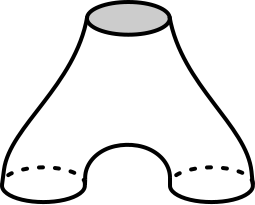
\includegraphics[scale=0.2]{../2020/pair-of-pants.png}}}
\end{equation}

\section{Prior Research}

\subsection{Neuro-Symbolic Integration}

There has been a long history of attempts to integrate symbolic logic with neural processing, with pioneers such as Ron Sun, Dov Gabbay, among others.  We consider 2 approaches below.

\textbf{Pascal Hitzler (\textit{et. al.})'s ``Core Method''} \cite{Hitzler2011} is model-based (as in model theory in logic).  An interpretation $\mathcal{I}$ is a function that assigns truth values to the set of all possible ground atoms.  To a logic program $P$ is associated a semantic operator $\mathcal{T}_P : \mathcal{I}_P \rightarrow \mathcal{I}_P$, where $\mathcal{I}_P$ is an interpretation endowed with the topology of the Cantor set.  Then $P$ is approximated by a neural network $f: \mathcal{I}_P \rightarrow \mathbb{R}$.

\textbf{Pedro Domingos' $\partial$-ILP} \cite{Domingos} is also model-based, and moreover it is focused on the learning problem.  A valuation is a vector $[0,1]^n$ mapping each ground atom to a real number $\in [0,1]$.  Each clause is attached with a Boolean flag (actually relaxed to be a continuous value) to indicate whether it is included in the results or not.  From each clause $c$ one can generate a function $\mathcal{F}_c$ on valuations that implements a single step of forward inference.  Then gradient descent is used to learn which clauses should be included.

The author believes that representing and learning relational knowledge is perhaps the final piece of the puzzle in AGI research.  We would like to mention a recent paper, \textbf{Geoffrey Hinton's GLOM theory} \cite{Hinton}, which addresses the problem of representing a hierarchy of visual structures.

\subsection{Cognitive Architectures and Reinforcement Learning}

\textbf{Reinforcement Learning (RL).}  In the 1980's, Richard Sutton \cite{Sutton1984} introduced reinforcement learning as an AI paradigm, drawing inspiration from Control Theory and Dynamic Programming.  In retrospect, RL already has sufficient generality to be considered an AGI theory, or at least as a top-level framework for describing AGI architectures.

\textbf{Relation to AIXI.}  AIXI is an abstract AGI model introduced by Marcus Hutter in 2000 \cite{Hutter2000}.  AIXI's environmental setting is the external ``world'' as observed by some sensors.  The agent's internal model is a universal Turing machine (UTM), and the optimal action is chosen by maximizing potential rewards over all programs of the UTM.  In our (minimal) model, the UTM is \uline{constrained} to be a neural network, where the NN's \textbf{state} is analogous to the UTM's \textbf{tape}, and the optimal weights (program) are found via Bellman optimality.

\textbf{Relation to Quantum mechanics and Path Integrals.}  At the core of RL is the Bellman equation, which governs the update of the utility function to reach its optimal value.  This equation (in discrete time) is equivalent to the Hamilton-Jacobi equation in differential form.  Nowadays they are unified as the Hamilton-Jacobi-Bellman equation, under the name ``optimal control theory'' \cite{Liberzon2012}.  In turn, the Hamilton-Jacobi equation is closely related to the Schr\"{o}dinger equation in quantum mechanics:
\begin{equation}
\boxed{\mbox{Bellman eqn.}} --- \boxed{\mbox{Hamilton-Jacobi eqn.}} --- \boxed{\mbox{Schr\"{o}dinger eqn.}}
\end{equation}
but the second link is merely ``heuristic'';  it is the well-studied ``quantization'' process whose meaning remains mysterious to this day.  Nevertheless, the path integral method introduced by Richard Feynmann can be applied to RL algorithms, eg. \cite{Kappen}.

The Hamilton-Jacobi equation gives the RL problem a ``symplectic'' structure;  Such problems are best solved by so-called symplectic integrators.  Surprisingly, in the RL / AI literature, which has witnessed tremendous growth in recent years, there is scarcely any mention of the Hamilton-Jacobi connection, while the most efficient heuristics (such as policy gradient, Actor-Critic, etc.) seem to exploit other structural characteristics of the ``world''.

\section{The Mathematical Structure of Logic}

Currently, the most mathematically advanced and satisfactory description of logic seems to base on category theory, known as categorial logic and topos theory.  This direction was pioneered by William Lawvere in the 1950-60's.  The body of work in this field is quite vast, but we shall briefly mention some points that are relevant to AGI.  A more detailed tutorial on categorical logic, with a focus on AGI, is in preparation \cite{Yan}.

\subsection{Predicates and Dependent Type Theory}

The Curry-Howard isomorphism identifies \textit{propositional} intuitionistic logic with type theory.  As such, the arrow $\rightarrow$ in type theory is ``used up'' (it corresponds to the implication arrow $\Rightarrow$ in intuitionistic logic).  However, predicates are also a kind of functions (arrows), so how could we accomodate predicates in type theory such that Curry-Howard continues to hold?  This is the idea behind Martin L\"{o}f's dependent type theory.

Predicate logic (in one form or another) is a highly desirable feature as AGI knowledge representation, due to its expressiveness.  So it seems necessary to incoporate dependent type theory into our logic.  From a categorical perspective, predicates can be regarded as \textbf{fibers} over a base set;  This is the treatment given by Bart Jacob's book \cite{Jacobs1999}.  The author has not yet mastered this knowledge adequately to say what implications it may have on AGI design, but it seems to offer an interesting angle.
%\begin{equation}
%\label{eqn:2-levels-of-TT}
%\vcenter{\hbox{\includegraphics[scale=0.5]{../2020/why-Martin-Lof.png}}}
%\end{equation}
%
%The type of $B$ in the dependent sum $\displaystyle \sum_A B$ depends on $A$. The sum of the entire family of $A$ (indexed by $B$) is similar to the product $A \times B$.
%
%The type of $B$ in the dependent product $\displaystyle \prod_A B$ depends on $A$. The product of the entire family of $A$ is similar to the exponentiation $B^A$.

\subsection{(Fuzzy?) Topos Theory}

The author's previous paper \cite{Yan2012} proposed a fuzzy-probabilistic logic where probabilities are distributed over fuzzy truth values.  To this day, he still believes that regarding fuzziness as a generalization of binary truth is philosophically sound.  Thus it behoves to develop a generalization of standard topos theory to the fuzzy case.  

The most important commutative diagram in Topos theory is this one:
\begin{equation}
\label{eqn:subobject-classifier}
\begin{tikzcd}[column sep = normal]
X \arrow[r, "!"] \arrow[d, tail, swap, "m"] & 1 \arrow[d, "\mathrm{true}"] \\
Y \arrow[r, swap, "\chi_m"] & \Omega
\end{tikzcd}
\end{equation}
It can be understood as saying that every set is a pullback of the true map, in analogy to the idea of a ``moduli space''.  Following this idea, is it true that every fuzzy set should be the pullback of the fuzzy true map?  It seems that the theory of fuzzy topos is still an open research problem \cite{}.

% The logic of sheaves is intuitionistic.

\section{Permutation Symmetry and Symmetric Neural Networks}
\label{sec:commutative-structure}

From the categorical perspective, we make the following correspondence with logic and type theory:
\begin{eqnarray}
\boxed{\mbox{product}} \quad A \times B \qquad & \leftrightsquigarrow & \qquad A \wedge B \quad \boxed{\mbox{conjunction}} \nonumber \\
\boxed{\mbox{function}} \quad A \rightarrow B \qquad & \leftrightsquigarrow & \qquad A \Rightarrow B \quad \boxed{\mbox{implication}}.
\end{eqnarray}
One basic characteristic of (classical) logic is that the conjuction $\wedge$ is \textbf{commutative}:
\begin{equation}
\mathsf{P} \wedge \mathsf{Q} \quad \Leftrightarrow \quad \mathsf{Q} \wedge \mathsf{P} .
\end{equation}
This remains true of probabilistic logic, where $\wedge$ and $\vee$ are unified as conditional probability tables (CPTs) for the nodes in Bayesian networks.

Once we know the symmetry, the question is how to impose this symmetry on deep neural networks.  Interestingly, the answer already comes from an independent line of research (namely, PointNet \cite{Qi2017a} and Deep Sets \cite{Zaheer2017a}) that deals with visual object recognition of point clouds:
\begin{equation}
\vcenter{\hbox{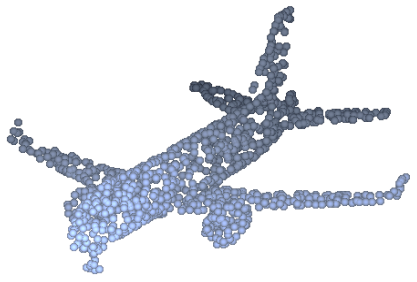
\includegraphics[scale=0.8]{point-cloud-aeroplane.png}}} \qquad
\vcenter{\hbox{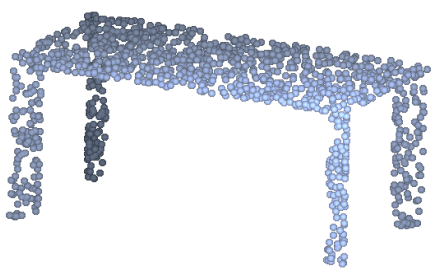
\includegraphics[scale=0.8]{point-cloud-desk.png}}}
\end{equation}
In a point cloud, it does not matter the order in which the points are presented, as inputs to the classifier function.  Such a function needs to be permutation invariant to a huge number of points.

From \cite{Zaheer2017a}: the \textbf{Kolmogorov–Arnold representation theorem} states that every multivariate continuous function can be represented as a sum of continuous functions of one variable:
\begin{equation}
f(x_1,... ,x_n) = \sum_{q=0}^{2n}\Phi_{q} \left(\sum_{p=1}^n \phi_{q,p}(x_p) \right)
\end{equation}
It can be specialized to such that every symmetric multivariate function can be represented as a sum of (the same) functions of one variable:
\begin{equation}
\label{symmetric-functions}
f(x_1, ..., x_n) = g(h(x_1) + ... + h(x_n))
\end{equation}
This leads to the following implementation using neural networks:
\begin{equation}
\vcenter{\hbox{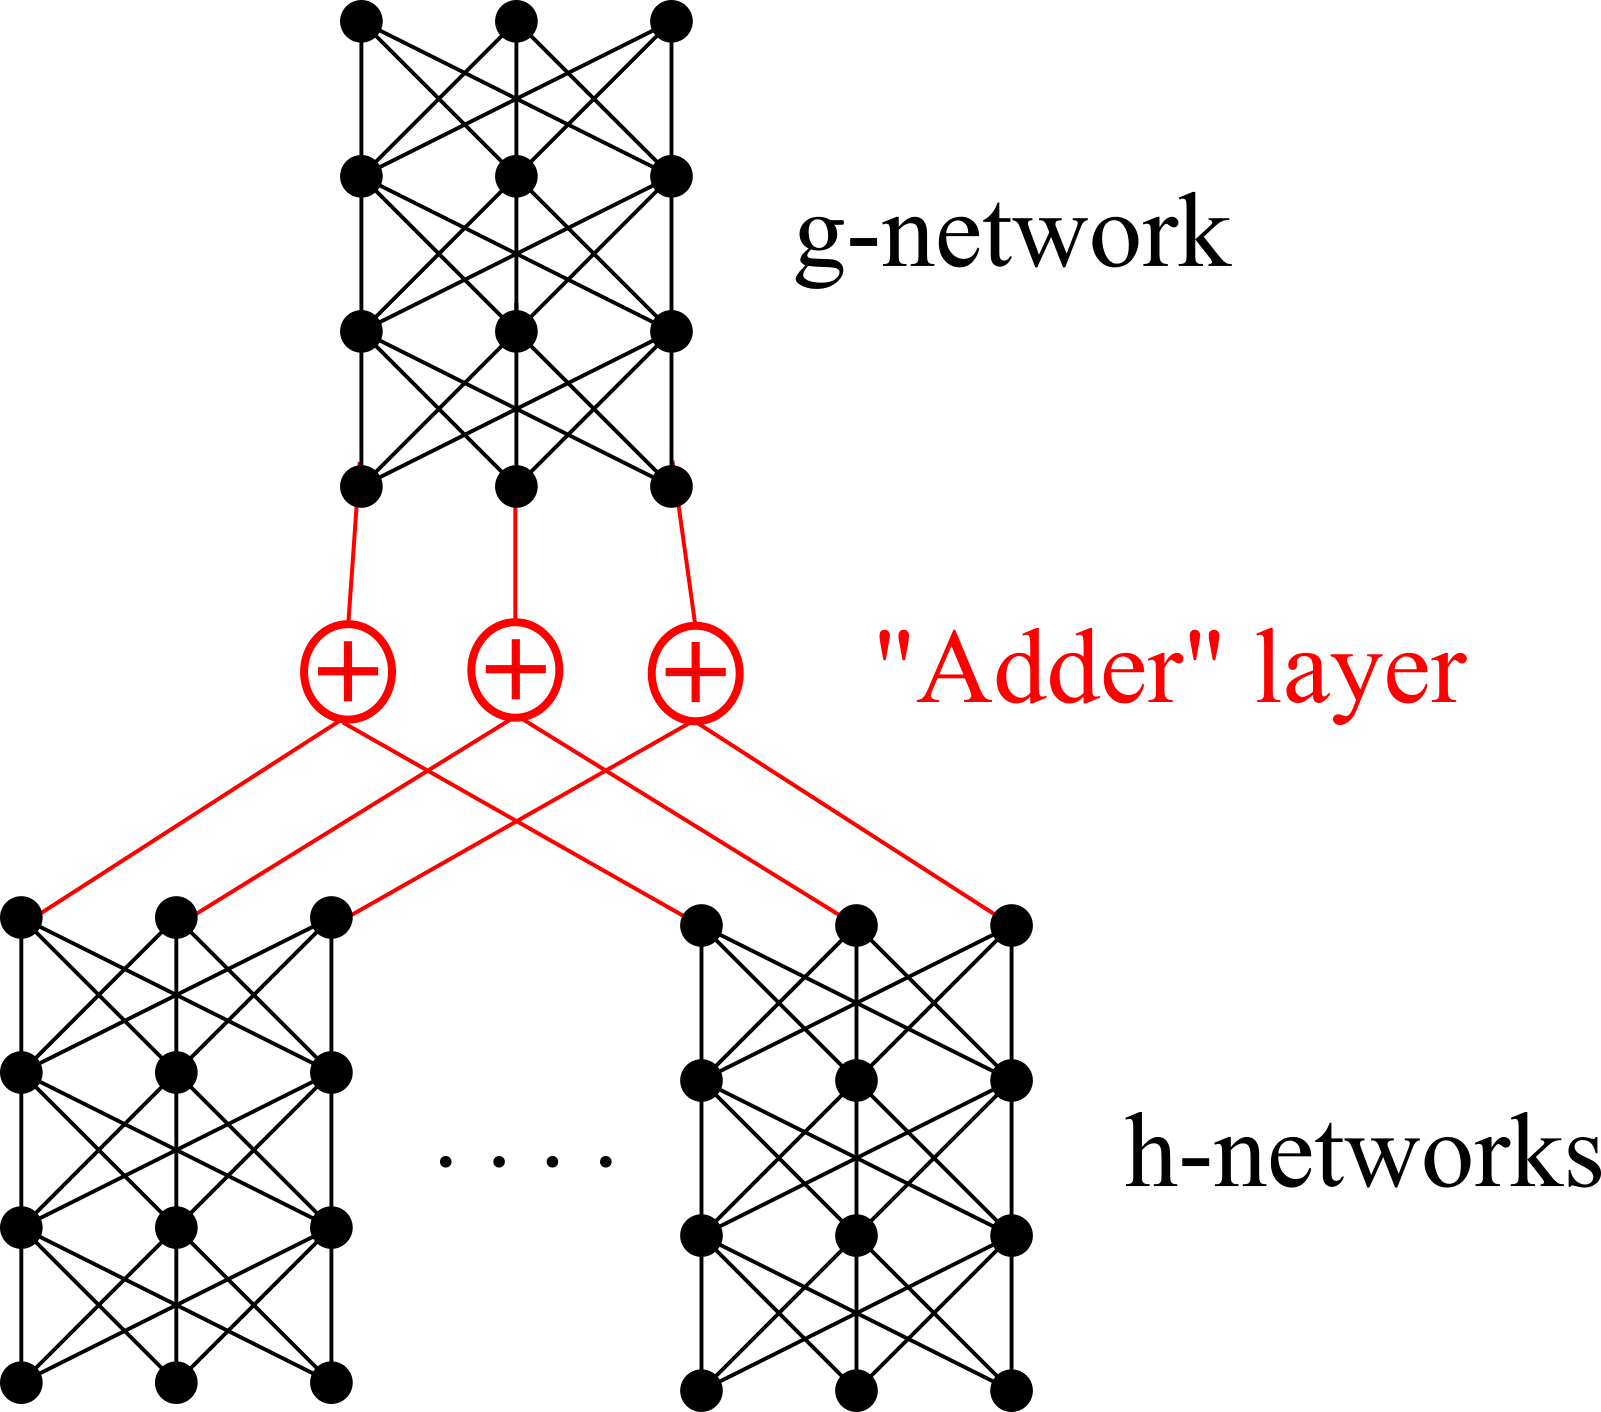
\includegraphics[scale=0.5]{g-and-h-networks.png}}}
\end{equation}
And this can be easily implemented with a few lines of Tensorflow (see \S\ref{sec:experiment}).

\subsection{Why BERT is a Logic}

In the following diagram, taken from \cite{}, observe that the Transformer is permutation-invariant (or more precisely, \textbf{equivariant}).  That is to say, for example, if input \#1 and \#2 are swapped, then output \#1 and \#2 would also be swapped:
\begin{equation}
\vcenter{\hbox{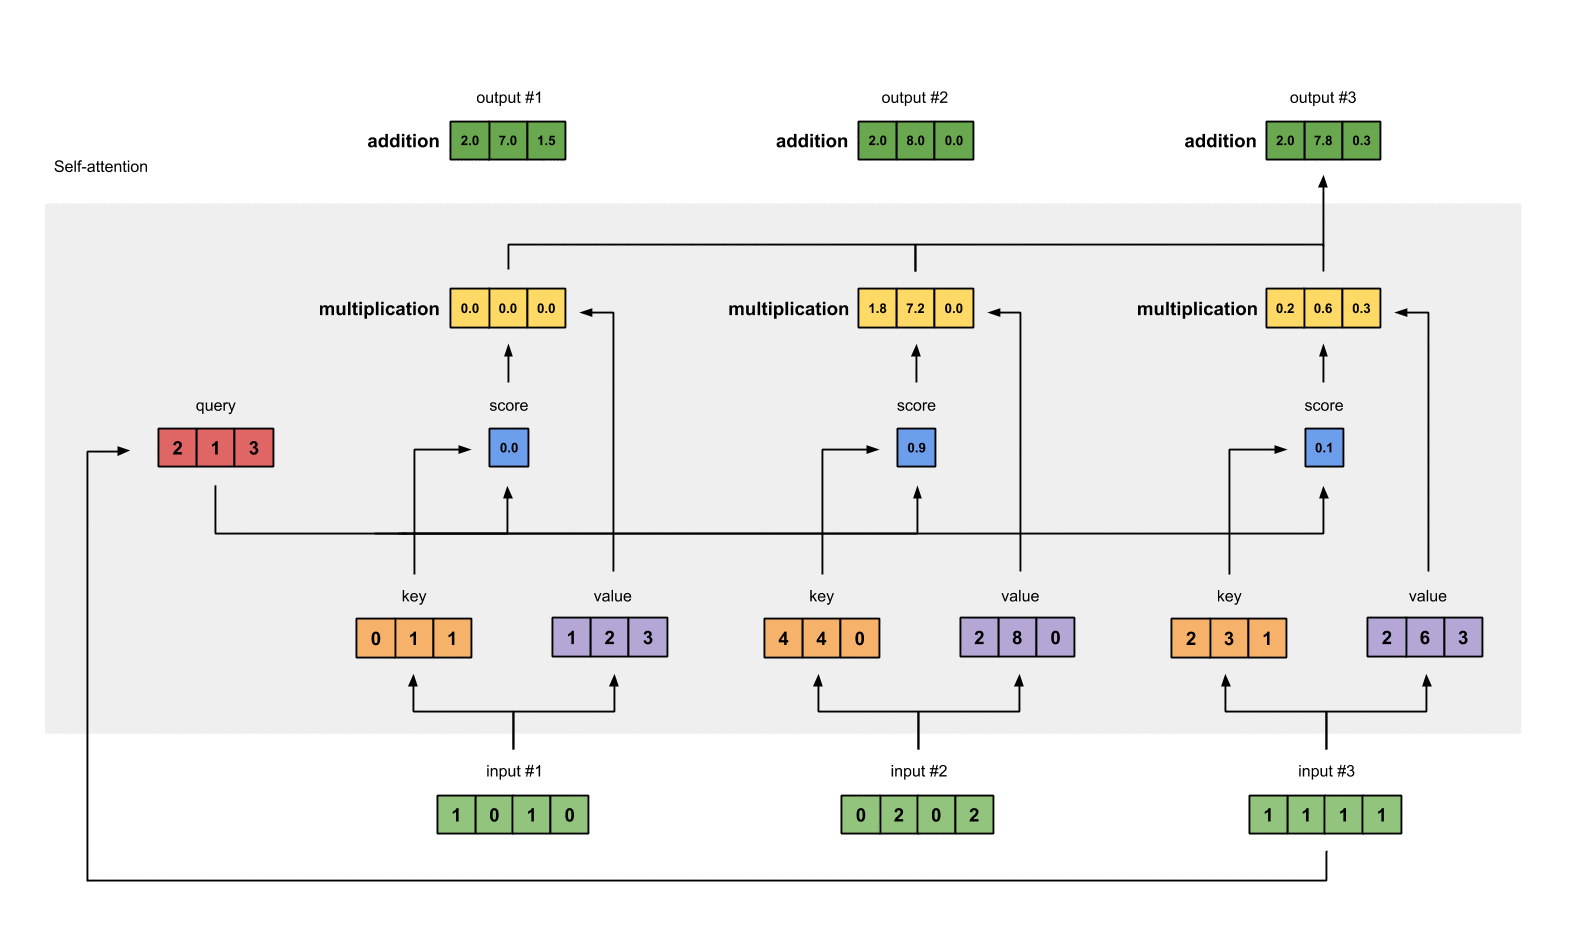
\includegraphics[scale=0.3]{self-attention.png}}}
\end{equation}
In other words, each Transformer layer takes $N$ inputs and produces $N$ equivariant outputs.  That is the same as saying that \textit{each} output is permutation-invariant in all its inputs.  As we explained in the last section, permutation invariance is the symmetry that characterizes a logic as having \textit{individual} propositions.

In \textbf{Multi-Head Attention}, the intermediate computations are duplicated multiple (eg, $M = 8$) times, each with their own weight matrices.  From the logic point of view, this amounts to duplicating $M$ logic rules per output.  But since the next layer still expects $N$ inputs, the $M$ outputs are combined into one, before the next stage.  Thus, from the logic point of view this merely increased the parameters \textit{within} a single logic rule, and seems not significant to increase the power of the logic rule-base.  Indeed, experimental results seem to confirm that multi-head attention is not particularly gainful towards performance.

A comment is in order here, about the choice of the word ``head''.  In logic programming (eg Prolog), one calls the conclusion of a logic rule its ``head'', such as \texttt{P} in \texttt{P :- Q,R,S}.  Perhaps the creators of BERT might have logic rules in mind?

\section{``No Free Lunch'' Theory}

The following conceptual diagram illustrates the possibility that there might exist some form of logic that is drastically different from the symbolic logic currently known to humans:
\begin{equation}
\vcenter{\hbox{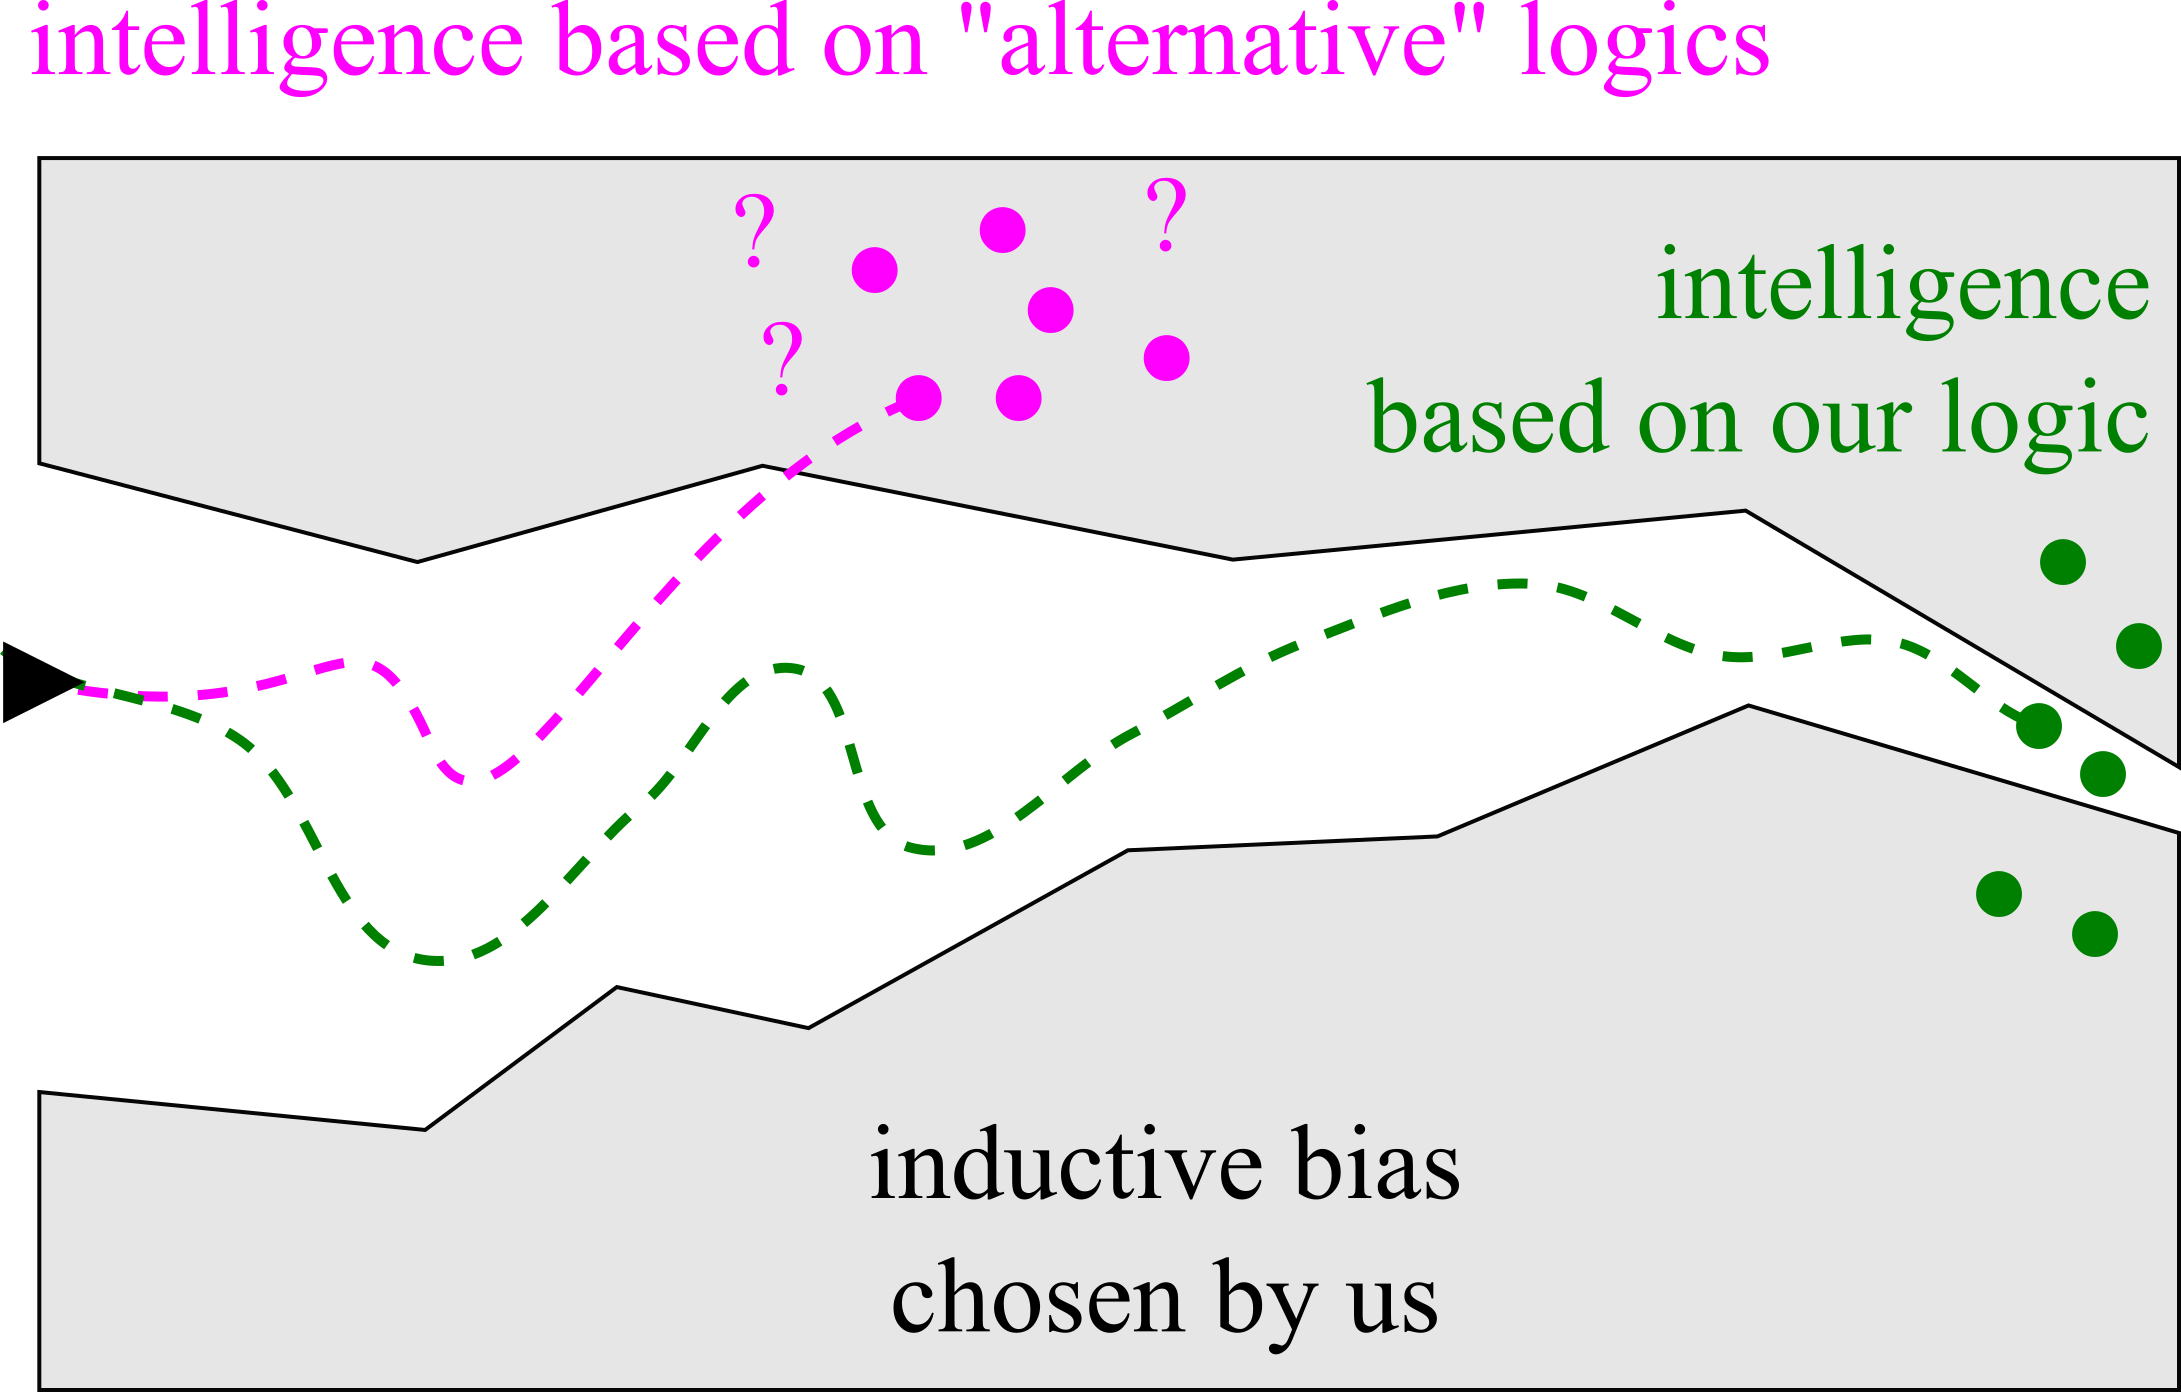
\includegraphics[scale=0.5]{no-free-lunch_Richard-Sutton.png}}}
\end{equation}
but there is no efficient algorithm to find them.  The permutation symmetry proposed in this paper forces our logic to be decomposable into \textbf{propositions}.  Such a logical form allows a mental state to be enumerated as a list of sentences (proposition), same as the ``linear'' nature of human \textbf{languages}.  If the AGI knowledge representation is linear (in the sequential sense) and symbolic, then it would not be far from our formulation -- all these logics belong to one big family.

But could there be drastically different logics?  One observes that pictures and music are not easily described by words, indeed they are 2-dimensional structures.  This suggests that the brain may use \textbf{multi-dimensional} matrices of features to represent the world.  Such a ``logic'' would be very different from sequential logic and it would be interesting and fruitful to analyze the relation between them.

\section{Experiment}
\label{sec:experiment}

A simple test of the symmetric neural network, under reinforcement learning (policy gradient), has been applied to the Tic-Tac-Toe game. \footnote{ Code with documentation is on GitHub: https://github.com/Cybernetic1/policy-gradient }

The state of the game is represented as a set of 9 propositions, where all the propositions are initialized as ``null'' propositions.  During each step of the game, a new proposition is added to the set (ie. over-writing the null propositions).  Each proposition encodes who the player is, and which square $(i,j)$ she has chosen.  In other words, it is a predicate of the form: \texttt{move(player,i,j)}.  The neural network takes all 9 propositions as input, and outputs a new proposition;  Thus it is a permutation-invariant function.

In comparison, the game state of traditional RL algorithms (eg. AlphaGo \cite{}) usually is represented as a vector of dimension same as the chessboard (eg. $3 \times 3$ in Tic-Tac-Toe and $8 \times 8$ in Chess).  This state vector remains the same constant length even if there are very few pieces on the chessboard.  Our logic-based representation may offer some advantages over the board-vector representation, and likely induces a different way of ``reasoning'' about the game.

In our Tic-Tac-Toe experiment, convergence of learning is observed, but the algorithm fell short of achieving the highest score (19 instead of 20), and the score displayed unstable oscillating behavior after it got near the optimal value.  Further investigation is required, but it seems to be a promising start.

\section{Conclusion and Future Directions}

We described a minimal AGI with a logic that can derive one new proposition per iteration.  This seems sufficient to solve simple logic problems such as Tic-Tac-Toe.  As a next step, we would consider inference rules with multi-proposition conclusions.  The latter seems essential to \textbf{abductive} reasoning.  For example, one can deduce the concept ``apple'' from an array of visual features;  Conversely, the idea of an ``apple'' could also evoke in the mind a multitude of features, such as color, texture, taste, and the facts such as that it is edible, is a fruit, and that Alan Turing died from eating a poisoned apple (a form of episodic memory recall), and so on.  This many-to-many inference bears some similarity to the brain's computational mechanisms \cite{Rolls} \cite{Rolls} \cite{Boraud}.  It may seem surprising, but there may exist a rough correspondence between the biological brain and a logic-baseed, reinforcement learning agent.  The author is embarking on an abstract unifying AGI theory that makes references to (but not necessarily copying) brain mechanisms.

\section*{Acknowledgements}

Thanks Ben Goertzel for suggesting that neural networks are advantageous over pure symbolic logic because they have fast learning algorithms (by gradient descent).  That was at a time when ``deep learning'' was not yet a popular word.  Thanks Dmitri Tkatch for pointing me to existing research of symmetric neural networks.  Thanks Dr. 肖达 (Da Xiao) for explaining details of BERT. 

Also thanks to the following people for invaluable discussions over many years:  Ben Goertzel, Pei Wang (王培), Abram Demski, Russell Wallace, Juan Carlos Kuri Pinto, SeH, Jonathan Yan, and others.  Also thanks to all the university professors and researchers in Hong Kong (especially in the math departments, and their guests), strangers who taught me things on Zhihu.com (知乎), Quora.com, and StackOverflow.

\printbibliography

\pagebreak

\section{Reinforcement-learning architecture}

The comparison of RL with neuroscience helps to crack the brain code:
\begin{itemize}
	\item What constitute the brain's \textbf{state}?
	\item What is the \textbf{state transition function}?
	\item What enables \textbf{learning} (in the state transtion function)?
\end{itemize}

We propose an AGI architecture:
\begin{enumerate}
	\item with \textbf{reinforcement learning} (RL) as top-level framework
	\begin{itemize}
		\item State space = mental space
		% \item Standard RL techniques can be employed to speed up learning (\S\ref{sec:policy-gradient})
	\end{itemize}
	\item \textbf{Logic} structure is imposed on the \textbf{knowledge representation} (KR)
	\begin{itemize}
		\item State transitions are given by logic rules = actions in RL
		\item The logic state $\vect{x}$ is decomposable into \textbf{propositions} (\S\ref{sec:LBAI-structure})
	\end{itemize}
	\item The set of logic rules is approximated by a deep neural network
	\begin{itemize}
		\item Just the most basic kind of feed-forward neural network (FFNN) is required
		\item Logic conjunctions are \textbf{commutative}, so working-memory elements can be presented in any order (\S\ref{sec:commutative-structure})
		\item \textbf{Stochastic} actions are represented by \textbf{Gaussian kernels} (radial basis functions) (\S\ref{sec:logic-actions}), thus partly avoiding the curse of dimensionality
	\end{itemize}
\end{enumerate}

The rest of this paper will explain these design features in detail.

The \textbf{metaphor} in the title of this paper is that of RL controlling an autonomous agent to navigate the maze of ``thoughts space'', seeking the optimal path:
\begin{equation}
\vcenter{\hbox{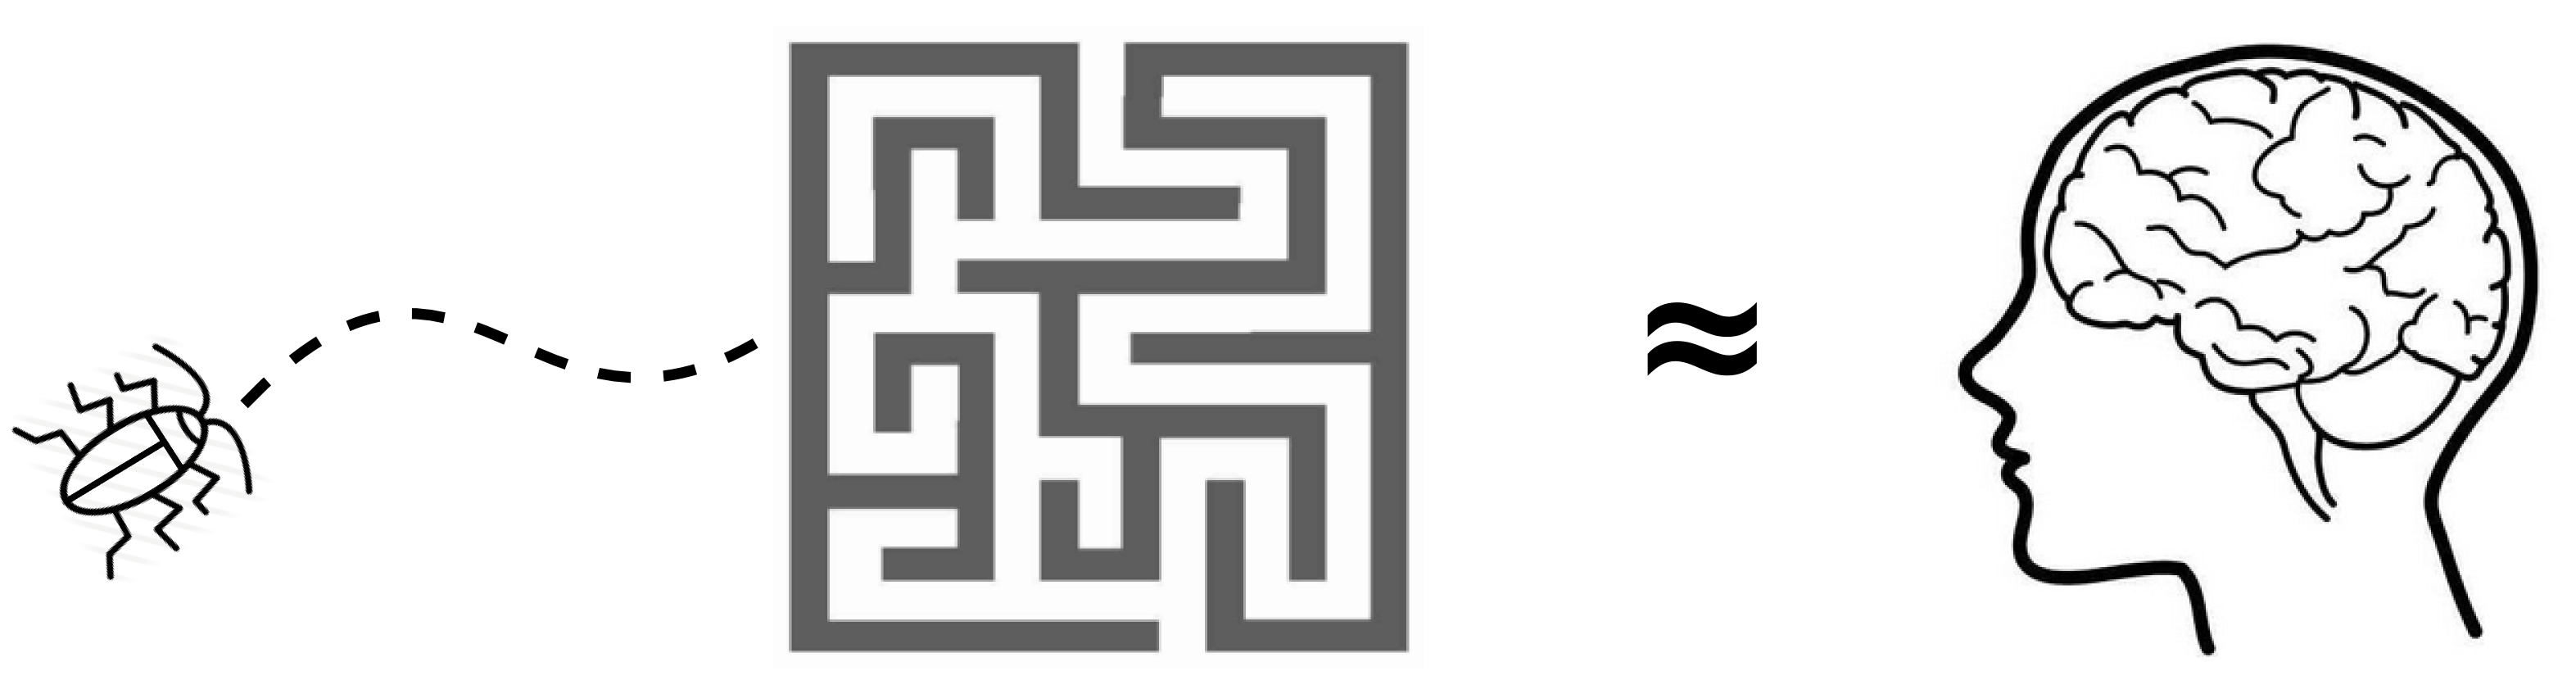
\includegraphics[scale=0.4]{maze-metaphor.png}}}
\end{equation}

The main idea is to regard ``thinking'' as a \emp{dynamical system} operating on \emp{mental states}:
\begin{equation}
\label{fig:mental-state}
\vcenter{\hbox{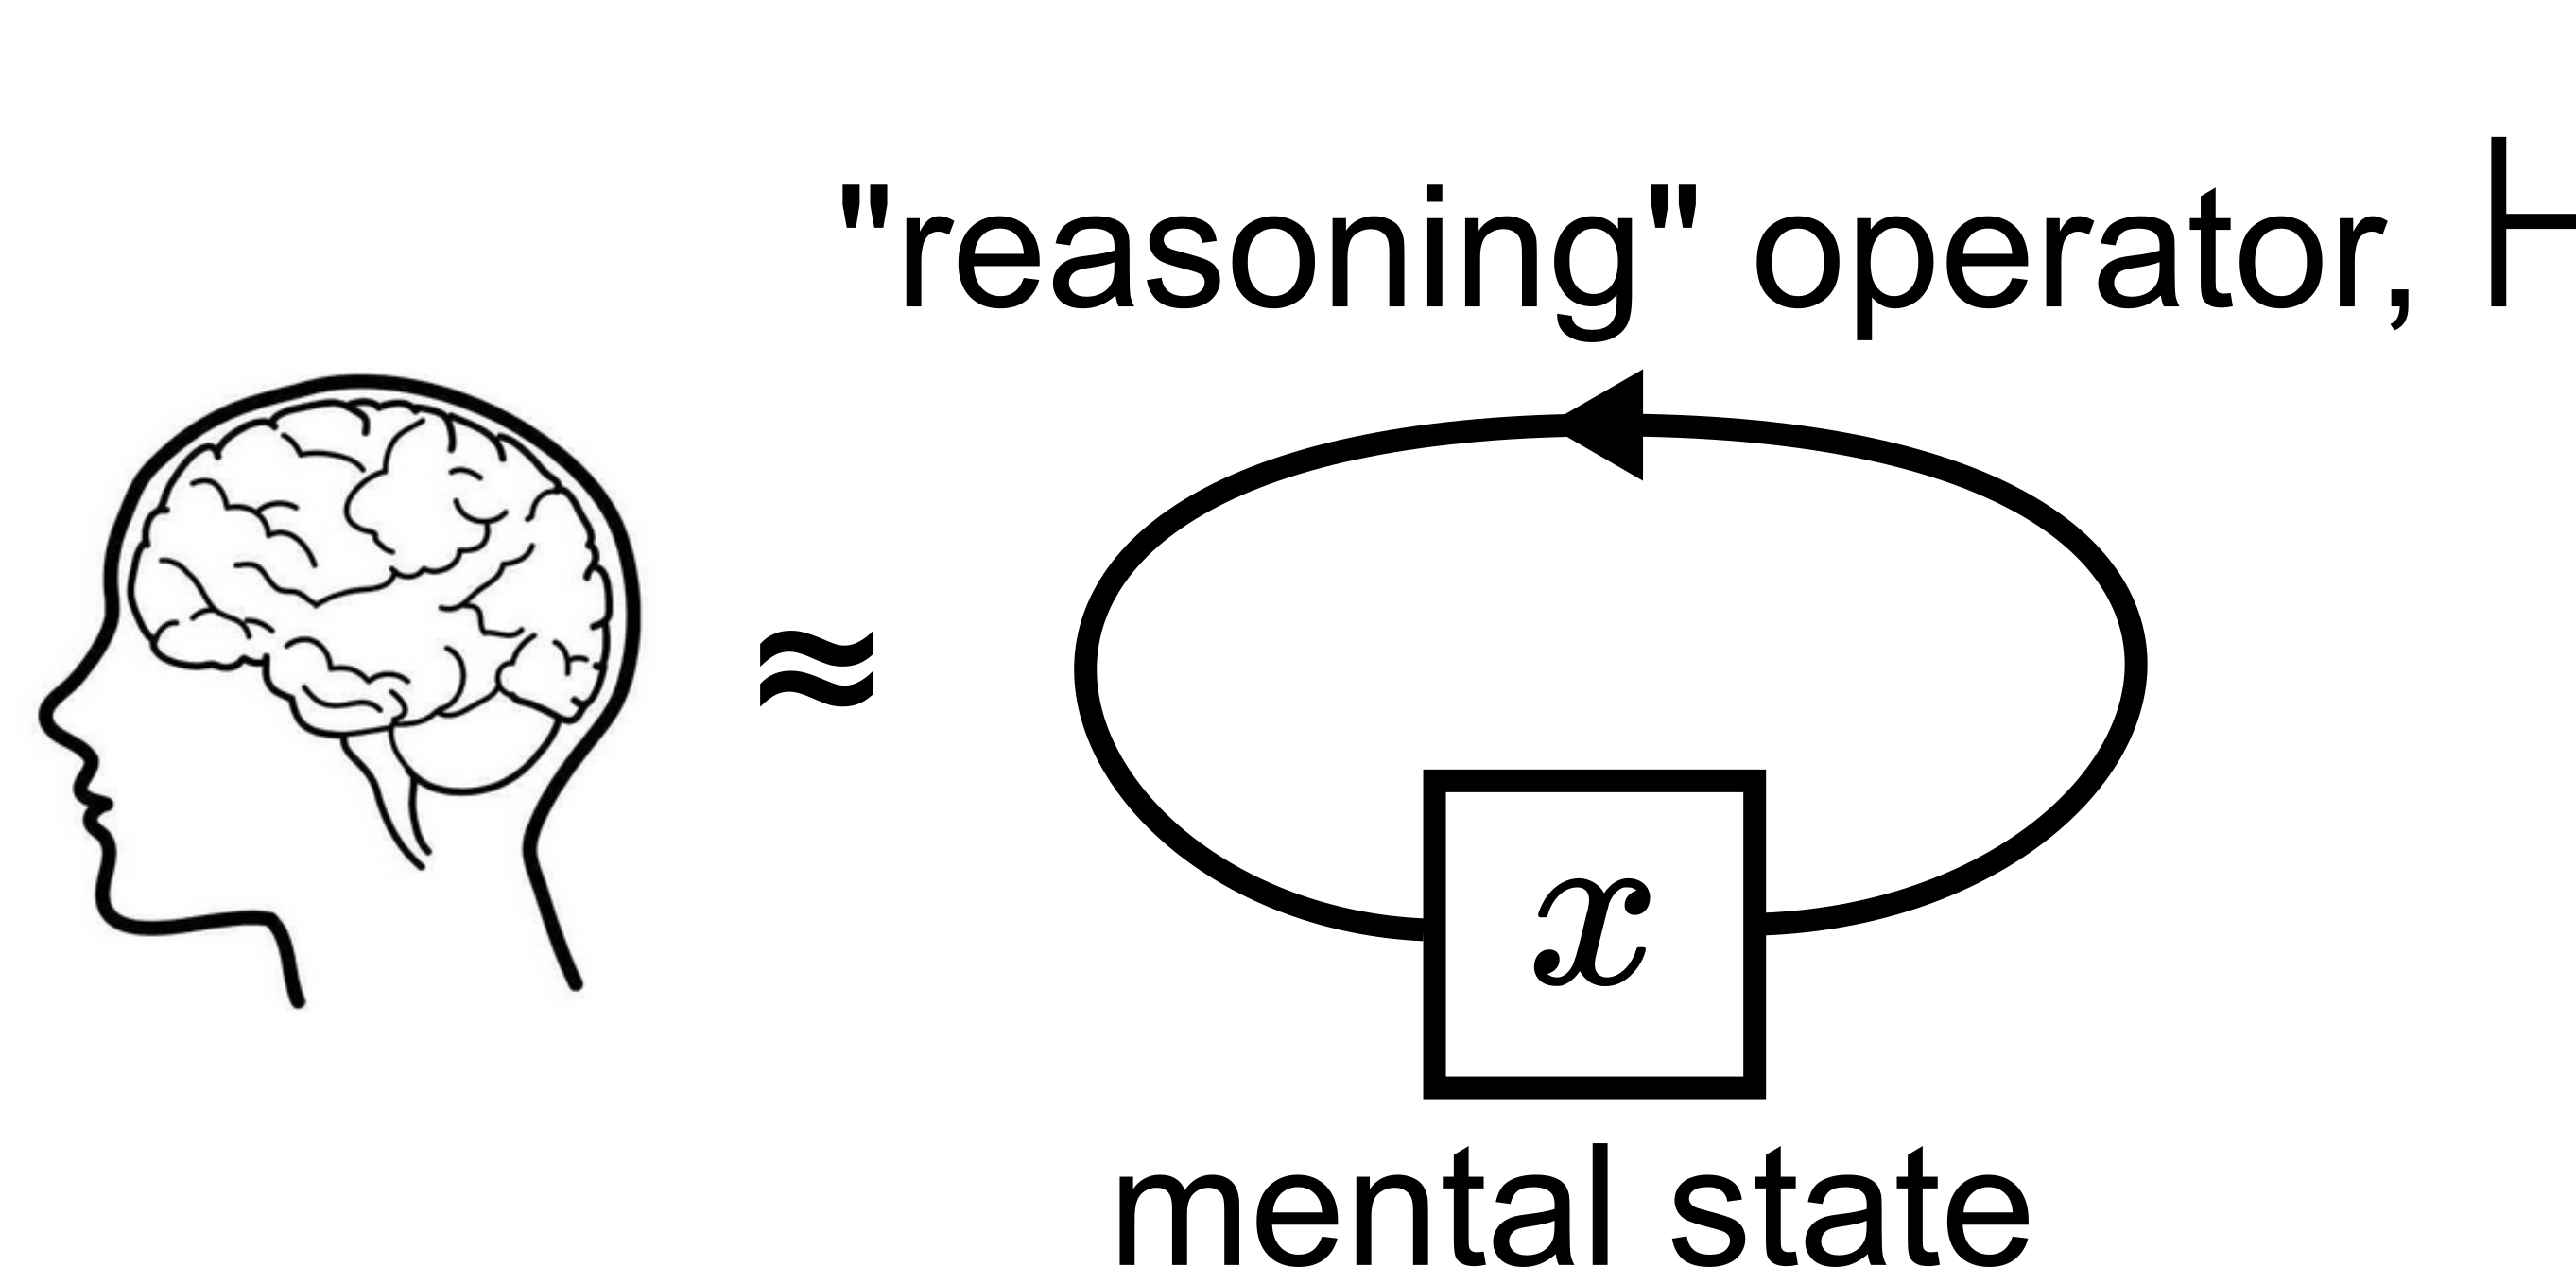
\includegraphics[scale=0.4]{mental-state.png}}}
\end{equation}

A mental state is a \textbf{set of propositions}, for example:
% \renewcommand{\labelitemi}{$\star$}
\begin{itemize}
\item I am in my room, writing a paper for AGI-2019.
\item I am in the midst of writing the sentence, ``I am in my room, ...''
\item I am about to write a gerund phrase ``writing a paper...''
\end{itemize}

Thinking is the process of \emp{transitioning} from one mental state to another.  As I am writing now, I use my mental states to keep track of where I am at within the sentence's syntax, so that I can construct my sentence grammatically.

%The following 3 disciplines are actually synonymous:
%\begin{itemize}
%\item in artificial intelligence, \textbf{reinforcement learning (RL)}
%\item in operations research, \textbf{dynamic programming}
%\item in modern control theory, the \textbf{state space} description
%\end{itemize}

%\begin{itemize}
%\item numerical optimization (eg gradient descent)
%\item differential equations governing time evolution
%\item dynamical systems theory, control theory, dynamic programming, reinforcement learning
% \item Lie algebra and $C^*$-algebra of continuous operators
% \item matrix theory, iteration and fixed-point theory
%\item neural networks and deep learning ... etc.
%\end{itemize}

%=======================================================================================
\begin{comment}

\subsection{Related work}

Google's \textbf{PageRank} is one of the earlier successful applications of vector-space and matrix techniques.  The \textbf{Word2Vec} \cite{Weston2015} algorithm that maps natural-language words to vectors is also spectacularly successful and influential;  it demonstrated the potential advantages of vector representations.  As for reinforcement learning, Q-learning (a form of RL) has been combined with deep learning to successfully play Atari games \cite{Mnih2013};  Their architecture is exactly the same as ours, except that we are trying to refine the internal structure of the learner.
%, both exploit the efficiency of vector and matrix calculus.

This is the cartoon version of our architecture:
\begin{equation}
\vcenter{\hbox{\includegraphics[scale=0.5]{architecture-cartoon.png}}}
\end{equation}

\subsection{``Introspective'' view of reinforcement learning}

Traditionally, RL deals with acting in an \textit{external} environment; value / utility is assigned to \textit{external} states.  In this view, the \textit{internal} mental state of the agent may change without any noticeable change externally:
\begin{equation}
\vcenter{\hbox{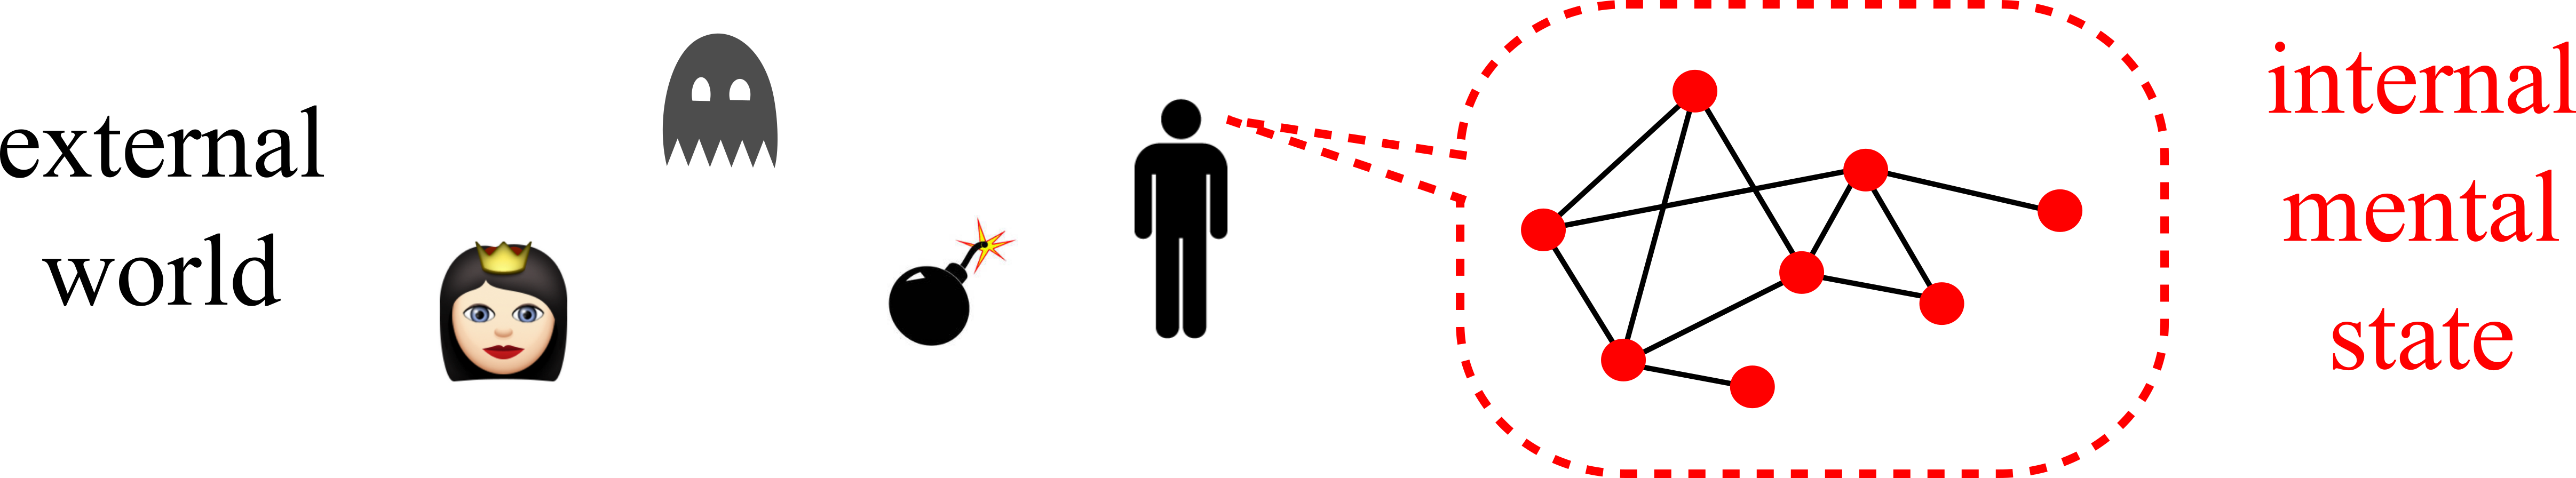
\includegraphics[scale=0.5]{save-princess.png}}}
\end{equation}
% The usefulness of RL (ie, the Bellman update technique) makes me wonder if it'd be advantageous to invert the perspective to consider the internal mental landscape instead.  Then, an internal state would have higher utility when it has been visited by many successful ``thinking'' trajectories.

%=======================================================================================
\end{comment}

\subsection{Actions = cognitive state-transitions = ``thinking''}

Our system consists of two main algorithms:
\begin{enumerate}
	\item Learning the transition function $\vdash$ or $\vect{F}: \vect{x} \mapsto \vect{x}'$.  $\vect{F}$ represents the \textbf{knowledge} that constrains thinking.  In other words, the learning of $\vect{F}$ is the learning of ``static'' knowledge.
	\item Transitioning from $\vect{x}$ to $\vect{x}'$.  This corresponds to ``thinking'' under the guidance of the static knowledge $\vect{F}$.
\end{enumerate}

In our architecture, $\vect{F}$ can be implemented as a simple feed-forward neural network (where ``deep'' simply means ``many layers''):
\begin{equation}
\vcenter{\hbox{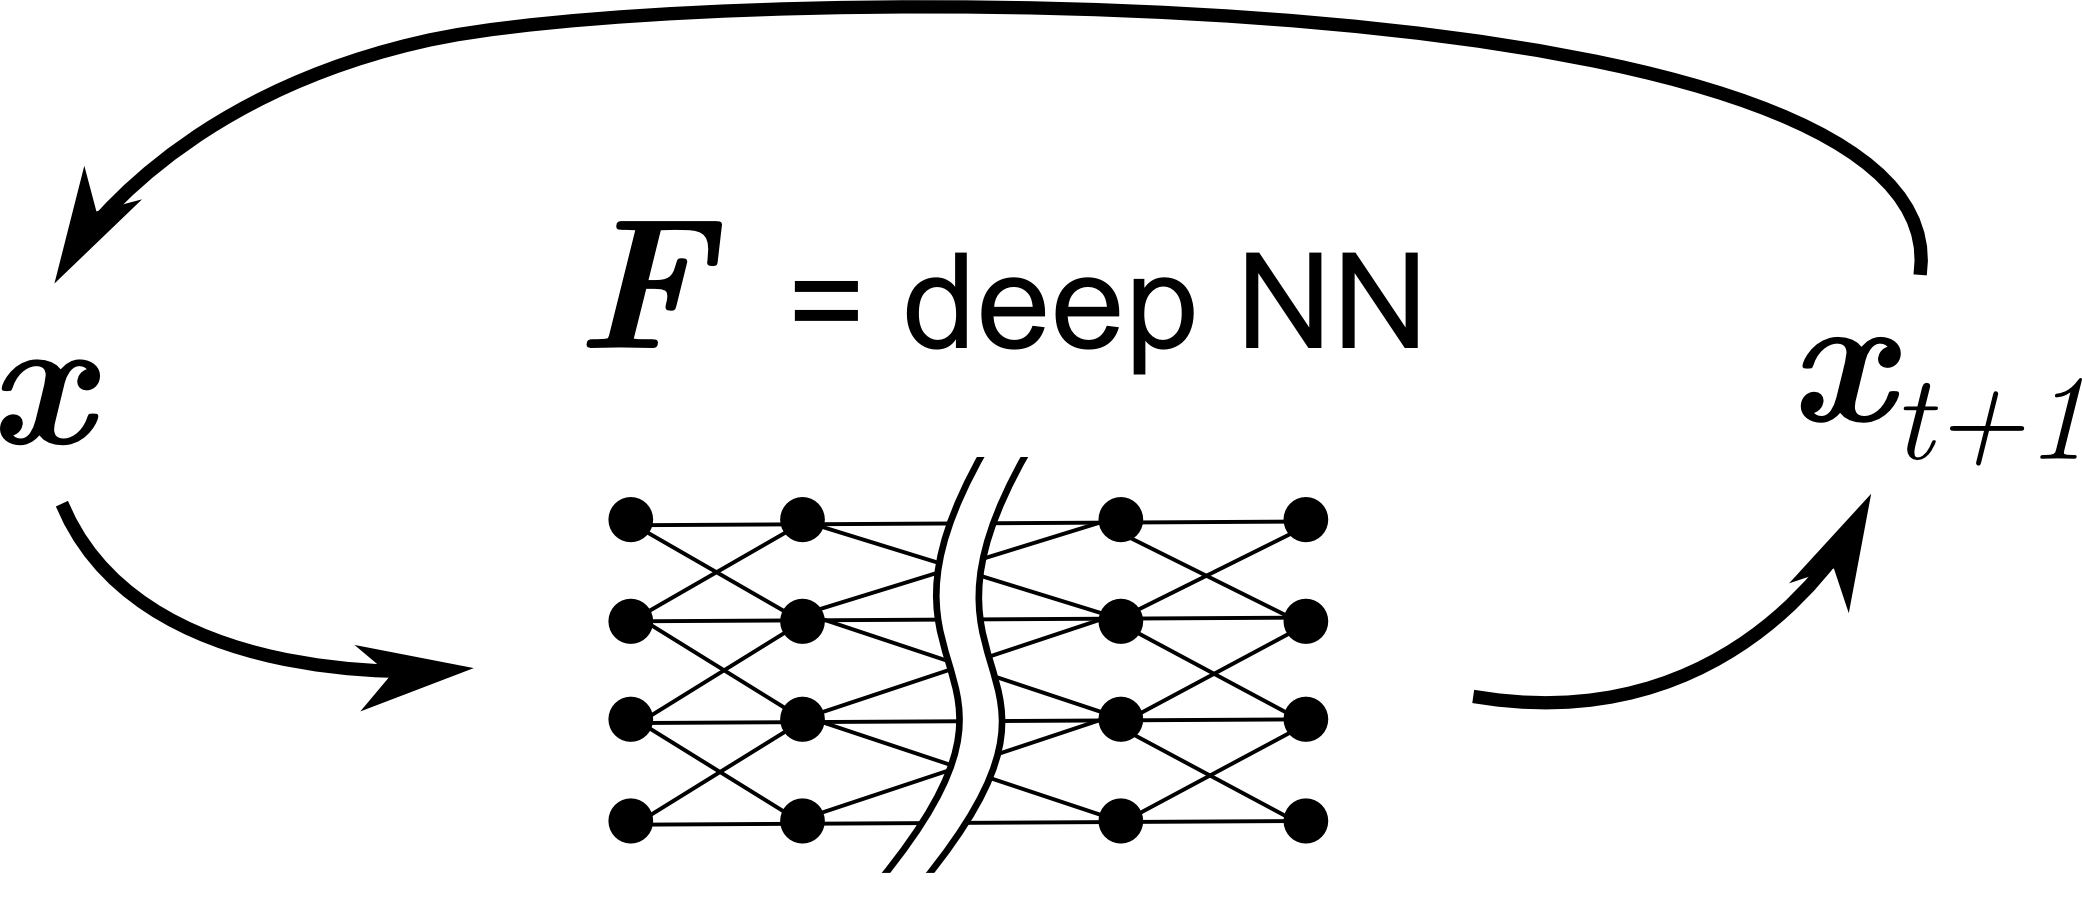
\includegraphics[scale=0.5]{genifer-model-00.png}}}
\label{eqn0}
\end{equation}
Since a recurrent NN is Turing-complete, this can be viewed as a minimalist AGI.  But its learning may be too slow without further \textbf{inductive bias} (\textit{cf} the ``no free lunch'' theorem \cite{Wikipedia-no-free-lunch}) --- so we will further modify $\vect{F}$ by imposing the logic structure of reasoning on it (\S\ref{sec:LBAI-structure} and \S\ref{sec:commutative-structure}).
% However, this naive idea has to be modified by the logic structures in \S\ref{sec:LBAI-structure} and \S\ref{sec:commutative-structure}.

In principle, every state is potentially \textbf{reachable} from every other state, if a logic rule exists between them.  Now we use a deep FFNN to represent the set of all logic rules.  This is a key efficiency-boosting step, because \uline{deep neural networks allows to use a polynomial number of parameters to represent an exponential number of mappings}.

Note that parts of the state $\vect{x}$ would be reserved and directly connect to the \textbf{input} and \textbf{output} of the AGI system.

%In this minimal architecture there is no \textbf{episodic memory}, but this does not seem to be a bottleneck problem. %\textit{The structure of memory} \cite{YanMemory}.

%\subsection{Constrained vs unconstrained dynamics}
%\label{sec:unconstrained-dynamics}

%In traditional reinforcement learning (left view), the system chooses an action $\vect{a}$, and the transition function $\vect{F}$ gives the probability of reaching each state $\vect{x}$ given action $\vect{a}$.  In our model (right view), all possible cognitive states are potentially \textbf{reachable} from any other state, and therefore the action $\vect{a}$ coincides with the next state $\vect{x}'$.

%In our formulation, every state is potentially \textbf{reachable} by some logic rule, this corresponds to the picture on the right:
%\begin{equation}
%\vcenter{\hbox{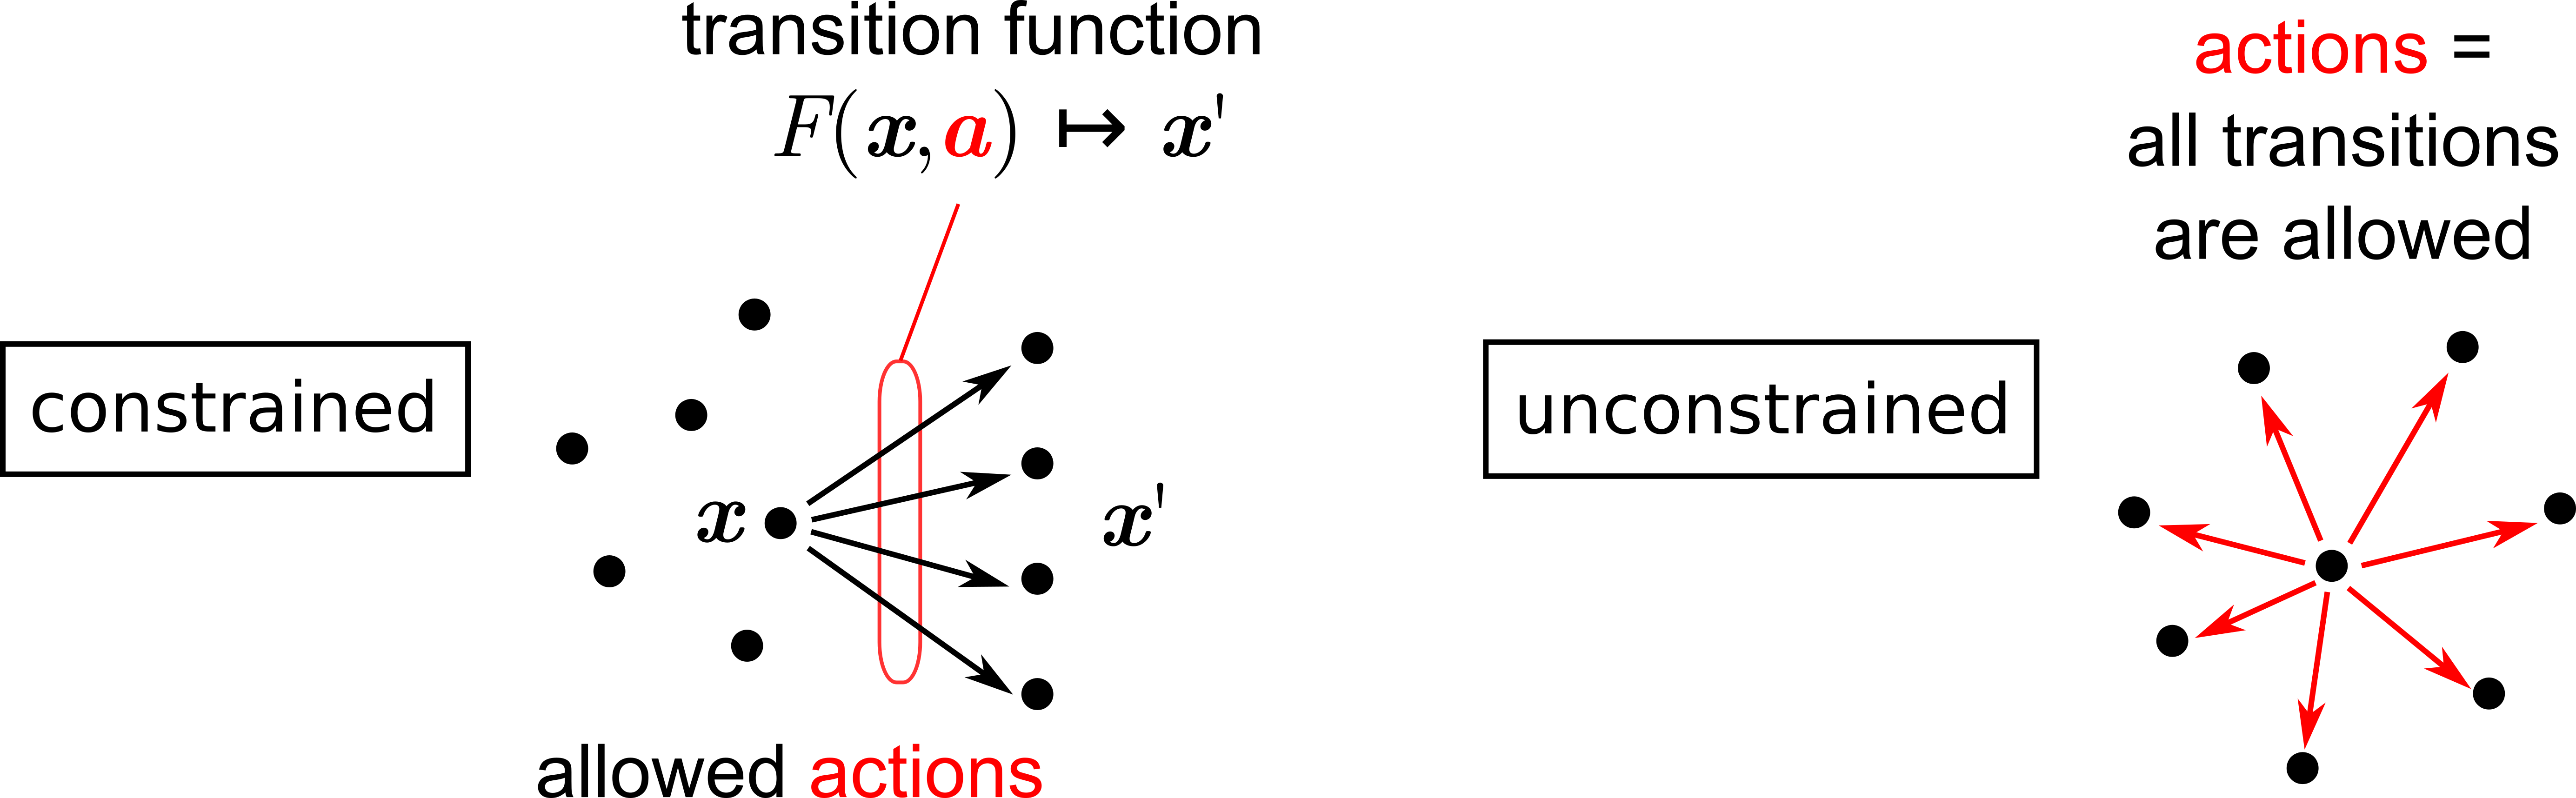
\includegraphics[scale=0.6]{Q-learning-2-views.png}}}
%\end{equation}

%Under this view, the control rule (\ref{eqn:control-rule}) simplifies to:
%\begin{equation}
%\dot{\vect{x}} = \vect{f}(\vect{x}, \vect{u}, t) = \vect{u}(t) .
%\end{equation}

%==================================================================================
\begin{comment}
and then the Lagrangian multiplier $\vect{\lambda} \equiv \vect{p}$ follows from (\ref{eqn:def-Hamiltonian}) and (\ref{eqn:variational-calculus}) to be:
\begin{equation}
\label{eqn:momentum}
\vect{\lambda}^* \equiv  \vect{p}^* = \frac{\partial L(t, \vect{x}^*, \vect{u}^*)}{\partial \vect{u}} = \frac{\partial L}{\partial \dot{\vect{x}}}
\end{equation}
which recovers the classical definition of \textbf{momemtum}.

Remember, the control-theoretic problem begins with the definition of the Lagrangian $L$ as a function of $(\vect{x}(t), \dot{\vect{x}}(t), t)$, where $\dot{\vect{x}} = \vect{u}$ in our unconstrained case.  In this setup, the concept of ``mass'' is unnecessary, but $L$ must be a function of $\dot{\vect{x}}$ (thus $\vect{u}$), or else the variational problem becomes trivial.  A crucial fact is that $L(\vect{x}(t), \vect{u}(t))$ is the same as $R(\vect{x} | \vect{a})$, ie, the \textbf{reward} obtained at state $\vect{x}$ after performing action $\vect{a}$.

The general procedure is to solve for the control $\vect{u}$ via the variational principle (\ref{eqn:variational-calculus}).  This leads to first solving for $\vect{p}$ via the \textbf{Euler-Lagrange equation}:
\begin{equation}
\frac{\partial L}{\partial \vect{x}} = \frac{d}{dt} \frac{\partial L}{\partial \dot{\vect{x}}} = \dot{\vect{p}} 
\end{equation}
which is basically Newton's $\vect{F} = m \vect{a}$.  Then we can solve for $\vect{u}$ via (\ref{eqn:momentum}).

\textbf{Symplectic} integrators preserve qualitatively the geometry of Hamiltonian flows. For example, the phase-space trajectory of a pendulum is a closed loop, but some integration methods such as \textbf{Runge-Kutta} may give trajectories that move towards the origin or diverge to $\infty$.

For more advanced theories on \textit{discrete} mechanics and control, \textit{cf} \cite{Marsden2001}, \cite{Lall2006}, \cite{Stern2008}, \textit{etc}.

%With the substitution $\Psi = e^{i U / \hbar}$ into the HJB equation, one can obtain the
%\emp{Schr\"{o}dinger equation}:
%\begin{equation}
%\boxed{\mbox{Schr\"{o}dinger}} \quad
%i \hbar \frac{\partial \Psi}{\partial t} = \hat{H} \Psi
%\end{equation}
%which means techiques in quantum mechanics can be applied to solve our AGI problem.

%==================================================================================
\end{comment}

\begin{comment}

\subsection{Control-theoretic setting}
\label{sec:control-theory}

The cognitive state is a vector $\vect{x} \in \mathbb{X}$ where $\mathbb{X}$ is the space of all possible cognitive states, the reasoning operator $\vdash$ or $\vect{F}$ is an \textbf{endomorphism} (an \textbf{iterative map}) $\mathbb{X} \rightarrow \mathbb{X}$.

Mathematically this is a \emp{dynamical system} that can be defined by:
\begin{eqnarray}
\boxed{\mbox{discrete time}} \quad \quad & \vect{x}_{t+1} = \vect{F}(\vect{x}_t) \label{eqn0}\\
\mbox{or } \boxed{\mbox{continuous time}} \quad \quad & \dot{\vect{x}} = \vect{f}(\vect{x}) \label{eqn1}
\end{eqnarray}
%($\vect{F}$ is implemented as the deep learning network in our approach.)
where $\vect{f}$ and $\vect{F}$ are different but related
\footnote{
	% They are related by: $\vect{x}(t + 1) = \vect{F}(\vect{x}(t))$, $\vect{x}^{-1}(\vect{x}(t)) = t =  \int^{\vect{x}_t}_{\vect{x}_0} \frac{d\vect{x}}{\vect{f}(\vect{x}(t))}$, and $f(\vect{x}) = \frac{1}{(\vect{x}^{-1})'(\vect{x}(t))}$.  So we can just solve the functional equation $\vect{x}^{-1}(\vect{F}(\vect{x})) - \vect{x}^{-1}(\vect{x}) = 1$. 
	See \textit{eg} \cite{Dolotin2007} \S8.2.3.
}.
For ease of discussion, sometimes I mix discrete-time and continuous-time notations.

A \emp{control system} is a dynamical system added with the control vector $\vect{u}(t)$:
\begin{equation}
\label{eqn:control-rule}
\dot{\vect{x}}(t) = \vect{f}(\vect{x}(t), {\color{red} \vect{u}(t)}, t) .
\end{equation}
The goal of control theory is to find the optimal $\vect{u}^*(t)$ function, such that the system moves from the initial state $\vect{x}_0$ to the terminal state $\vect{x_\bot}$.

\end{comment}

\begin{comment}
A typical control-theory problem is described by:
\begin{eqnarray}
\boxed{\mbox{state equation}} \quad & \dot{\vect{x}}(t) = \vect{f}[\vect{x}(t), \vect{u}(t), t] \label{eqn1}\\
\boxed{\mbox{boundary condition}} \quad & \vect{x}(t_0) = \vect{x}_0 \,,\, \vect{x}(t_\bot) = \vect{x}_\bot \\
\boxed{\mbox{objective function}} \quad & J = \int_{t_0}^{t_\bot} L[\vect{x}(t), \vect{u}(t), t] dt
\end{eqnarray}
and we seek the optimal control $\vect{u}^*(t)$.
\end{comment}

%According to control theory, the condition for \textbf{optimal path} is given by the Hamilton-Jacobi-Bellman equation:
%\begin{equation}
%\boxed{\mbox{Hamilton-Jacobi-Bellman}} \quad
%0 = \frac{\partial J^*}{\partial t} + \min_u H
%\end{equation}
%\frac{d}{dt} V(x,t) = \min_u \{ C(x,u) + \langle \nabla V(x,t), f(x,u) \rangle \} 

% In the next section %\S\ref{sec:quantum}
% we shall look into the meaning of $J$, $L$, and $H$.

\begin{comment}
\subsection{Reinforcement learning / dynamic programming}

\textbf{Reinforcement learning} is a branch of machine learning that is particularly suitable for controlling an \textbf{autonomous agent} who interacts with an \textbf{environment}.  It uses \textbf{sensory perception} and \textbf{rewards} to continually modify its \textbf{behavior}.  The exemplary image you should invoke in mind is that of a small insect that navigates a maze looking for food and avoiding predators:  $\vcenter{\hbox{\includegraphics[scale=0.1]{cockroach.png}}}$

A reinforcement learning system consists of a 4-tuple:
\begin{equation}
\boxed{\mbox{reinforcement learning system}} \; = (\vect{x} \in \mbox{States}, \vect{u} \in \mbox{Actions}, R = \mbox{Rewards}, \pi = \mbox{Policy})
\end{equation}
For details readers may see my \textit{Reinforcement learning tutorial} \cite{YanRLtutorialEN}.

%is synonymous with \textbf{dynamic programming}, which is also the main content of modern \textbf{control theory} with the state-space description.

$U$ is the total rewards of a sequence of actions:
%\begin{equation}
%\boxed{\mbox{total value of state 0}} \; U(\vect{x}_0) = \sum_t \; \boxed{\mbox{reward at time t}} \; R(\vect{x}_t, \vect{u}_t)
%\end{equation}
\begin{eqnarray}
\mbox{\footnotesize total value of state 0} \tikzmark{uu} & \quad \quad \quad & \mbox{\footnotesize reward at time $t$} \tikzmark{rr} \nonumber \\
\nonumber \\
\tikzmark{UU} U(\vect{x}_0) & = & \sum_t \; \tikzmark{RR} R(\vect{x}_t, \vect{u}_t)
\begin{tikzpicture}[overlay,remember picture]
  \draw (uu.center) +(-50pt,-3pt) -- ([shift={(4pt,12pt)}]UU.center);
  \draw (rr.center) +(-35pt,-3pt) -- ([shift={(8pt,12pt)}]RR.center);
\end{tikzpicture}
\end{eqnarray}
For example, the value of playing a chess move is not just the immediate reward of that move, but includes the consequences of playing that move (eg, greedily taking a pawn now may lead to checkmate 10 moves later).  Or, faced with delicious food, some people may choose not to eat, for fear of getting fat.

%The goal of \textbf{reinforcement learning} is to learn the \emp{policy function}:
%\begin{equation}
%\begin{tikzcd}[]
%\mbox{policy : ~~state} \arrow[r, mapsto, "\scalebox{0.8}{action}"] & \mbox{state'}
%\end{tikzcd}
%\end{equation}
%when we are given the \emp{state space}, \emp{action space}, and \emp{reward function}:
%\begin{equation}
%\mbox{reward}: \boxed{\mbox{state}} \times \boxed{\mbox{action}} \rightarrow \mathbb{R}
%\end{equation}
%The action $a$ is the same notion as the control variable $u$ in control theory.

The central idea of \textbf{Dynamic programming} is the \textbf{Bellman optimality condition}, % Richard Bellman in 1953 proposed this formula, while he was working at RAND corporation, dealing with operations research problems.
% The \textbf{Bellman condition} 
which says:  ``\uline{if we cut off a tiny bit from the endpoint of the optimal path, the remaining path is still an optimal path between the new endpoints}.''

\begin{eqnarray}
& \mbox{\footnotesize value of entire path} \tikzmark{uEntire} \quad \quad \mbox{\footnotesize reward of choosing $\vect{u}$ at current state} \tikzmark{rCurrent} \quad \quad \mbox{\footnotesize value of rest of path} \tikzmark{uRest} \nonumber \\
\nonumber \\
& \boxed{\mbox{Bellman equation}} \quad \tikzmark{UEntire} U^*(\vect{x}) = \max\limits_{\vect{u}} \{ \; \tikzmark{RCurrent} R(\vect{u}) + \tikzmark{URest} U^*(\vect{x}_{t+1}) \; \}
\begin{tikzpicture}[overlay,remember picture]
  \draw (uEntire.center) +(-30pt,-3pt) -- ([shift={(4pt,12pt)}]UEntire.center);
  \draw (rCurrent.center) +(-80pt,-3pt) -- ([shift={(4pt,12pt)}]RCurrent.center);
  \draw (uRest.center) +(-65pt,-3pt) -- ([shift={(8pt,12pt)}]URest.center);
\end{tikzpicture}
\end{eqnarray}
This seemingly simple formula is the \uline{entire content} of dynamic programming;  What it means is that:  When seeking the path with the best value, we cut off a bit from the path, thus reducing the problem to a smaller problem;  In other words, it is a \textbf{recursive relation} over time.

In AI reinforcement learning there is an oft-employed trick known as $Q$-learning.  $Q$ value is just a variation of $U$ value;  there is a $U$ value for each state, and $Q$ is the \textbf{decomposition} of $U$ by all the actions available to that state.  In other words, $Q$ is the utility of doing action $\vect{u}$ in state $\vect{x}$.  The relation between $Q$ and $U$ is:
\begin{equation}
U(\vect{x}) = \max\limits_{\vect{u}} \, Q(\vect{x}, \vect{u})
\end{equation}
The advantage of $Q$ is the ease of learning.  We just need to learn the value of actions under each state.  This is so-called ``\textbf{model free learning}''.

%The \emp{Bellman equation} governs reinforcement learning just as in control theory:
%\begin{eqnarray}
%\boxed{\mbox{optimal path}} = & \mbox{choose max reward on current path segment} \nonumber \\
%& \quad + \boxed{\mbox{the rest of optimal path}}
%\end{eqnarray}
%In math notation:
%\begin{equation}
%U^*_t = \max_{u} \{ \; \boxed{\mbox{reward}(u, t)} + U^*_{t-1} \; \}
%\end{equation}
%where $U$ is the ``long-term value'' or \emp{utility} of a path.

%Conceptually, $U$ is the \textbf{integration} of instantaneous rewards over time:
%\begin{equation}
%\boxed{\mbox{utility, or value} U} = \int \boxed{\mbox{reward} R} \,dt
%\end{equation}
\end{comment}

\begin{comment}
%==================================================================================
Under the reinforcement learning framework, intelligence is decomposed into \textbf{thinking} and \textbf{learning}:
\begin{itemize}
\item \emp{Thinking} means finding the optimal trajectory of $\vect{x}$ according to the \textbf{knowledge} stored in the deep NN.  This is achieved using the Bellman equation to calculate $\vect{u}^*$.  The trajectory of $\vect{x}$ is constrained by the deep NN (in other words, the system must think in accordance with \textbf{correct knowledge}).  While thinking, the deep NN stays \textbf{constant}.

\item \emp{Learning} means learning the weights in the deep NN.  Changing $W$ changes $\vect{F}$, which determines the state equation (\ref{eqn0}), so the entire system becomes a new one.  In other words, deep NN learning is a kind of \textbf{second-order learning}:  Consider 2 systems $\vect{F}$ and $\vect{F} + \epsilon \hat{\vect{F}}$, after \uline{many trials} of thinking with different premises, if the average reward is higher in the altered system, $\vect{F}$ will learn towards the $\hat{\vect{F}}$ direction.
% 即是根据已学得的\textbf{知识}(知识储存在 deep NN 里),在思维空间中找寻 $\vect{x}$ 最优的轨迹,方法是根据 Bellman 方程计算 $\vect{u}^*$。 $\vect{x}$ 的轨迹受 deep NN 约束(亦即是说,系统只能依据\textbf{正确的知识}去思考),思考时 deep NN 是\textbf{不变}的。
%\item \emp{学习}就是学习神经网络 deep NN 的 weights $W_\ell$,改变 $W$ 即改变 $\vect{F}$,而$\vect{F}$ 决定\textbf{状态方程} (\ref{eqn0}),所以整个系统变了另一个系统。 换句话说,deep NN 的学习是一种 \textbf{second-order learning}: 考虑两个系统 $\vect{F}$ 和 $\vect{F} + \epsilon \hat{\vect{F}}$,经过很多次思考过程,如果奖励的平均值在后者有所增加,则 $\vect{F}$ 向 $\hat{\vect{F}}$ 方向学习。
\end{itemize}
%==================================================================================
\end{comment}

%=======================================================================================
\begin{comment}

\subsection{Lagrangians and Hamiltonians}
\label{sec:Langrangians-Hamiltonians}
%\subsection{Control theory / dynamical systems theory}

%This section is optional.

In \emp{reinforcement learning}, we are concerned with two quantities:
\begin{itemize}
	\item $r(\vect{x}, \vect{u})$ = \emp{reward} of doing action $\vect{u}$ in state $\vect{x}$
	\item $U(\vect{x})$ = \emp{utility} or \emp{value} of state $\vect{x}$ 
\end{itemize}
where \textbf{utility} is the integral of instantaneous \textbf{rewards} over time:
\begin{equation}
\boxed{\mbox{utility} $U$} = \int \boxed{\mbox{reward} $r$} \,dt .
\end{equation}
%(价值有时用 $V$ 表示,但为避免和势能 $V$ 混淆故不用。)

%In \emp{control-theoretic} parlance, it is usually defined the \textbf{cost functional}:
%\begin{equation}
%\boxed{\mbox{cost } $J$} = \int L dt + \Phi(\vect{x}_\bot)
%\end{equation}
%where $L$ is the \textbf{running cost}, ie, the cost of making each step; 
%$\Phi$ is the \textbf{terminal cost}, ie, the value when the terminal state $\vect{x}_\bot$ is reached.

%Define a continuous version of ``utility'':
%\begin{equation}
%V(x,t) = \min_u \{ \int_t^{t_\bot} C(x,u)dt + \Phi(x_\bot,t_\bot) \} 
%\end{equation}
%where $t$ is time, $u$ is a set of control parameters, $C$ is the \emp{cost-rate} function:
%\begin{equation}
%\int C dt = R = \mbox{reward}
%\end{equation}
%This integral expresses the ``cost of the path'', whereas $\Phi(x_\bot,t_\bot)$ is the ``cost at termination''.

%In \emp{analytical mechanics} $L$ is known as the \textbf{Lagrangian}, and the time-integral of $L$ is called the \textbf{action}:
%\begin{equation}
%\boxed{\mbox{action } $S$} = \int L dt
%\end{equation}
%Hamilton's \emp{principle of least action} says that $S$ always takes the \textbf{stationary value}, ie, the $S$ value is extremal compared with neighboring trajectories.

%The \textbf{Hamiltonian} is defined as $\displaystyle H = L + \frac{\partial J^*}{\partial \vect{x}} \vect{f}$, which arises from the method of \textbf{Lagrange multipliers}.  % For details please refer to my \textit{Control theory tutorial}\cite{YanControlTheoryTutorial}.

%All these refer to essentially the same thing, so we have the following correspondence:

There is a well-known correspondence between control theory, dynamic programming (reinforcement learning), and analytical mechanics, observed by Kalman and Pontryagin, among others (\textit{cf} the textbook \cite{Liberzon2012}):
\setlength{\tabcolsep}{0.5em} % for the horizontal padding
{\renewcommand{\arraystretch}{1.2}
\begin{equation}
\begin{tabular}{|c|c|c|}
\hline 
\emp{Reinforcement learning} & \emp{Control theory} & \emp{Analytical mechanics} \\ 
\hline
value $V$ or utility $U$ & cost $J$ & action $S$ \\ 
\hline 
instantaneous reward $r$ & running cost $L$ & Lagrangian $L$ \\ 
\hline 
action $\vect{a}$ & control $\vect{u}$ & (external force) \\
\hline
 & Lagrange multiplier $\vect{\lambda}$ & momentum $\vect{p}$ \\
\hline
$ U = \int R \,dt$ & $ J = \int L \,dt + \Phi(\vect{x}_\bot)$ & $ S = \int L \,dt$ \\
\hline
\end{tabular} 
\end{equation}
}
$\Phi$ is the \textbf{terminal cost}, ie, the value when the terminal state $\vect{x}_\bot$ is reached.

Interestingly, the reward $r$ corresponds to the \textbf{Lagrangian} in physics, whose unit is ``energy'';  In other words, ``desires'' or ``happiness'' appear to be measured by units of ``energy'', this coincides with the idea of ``positive energy'' in pop psychology.  Whereas, long-term value is measured in units of $[\mbox{energy} \times \mbox{time}]$.

The \textbf{Hamiltonian} can be defined by
\begin{equation}
\label{eqn:def-Hamiltonian}
H := \langle \vect{p}, \vect{f} \rangle - L
\end{equation}
which arises from the \textbf{Lagrange multiplier} $\vect{\lambda} \equiv \vect{p}$.  It can be shown that, at the optimum,
\begin{equation}
\vect{\lambda} = \frac{\partial J^*}{\partial \vect{x}}
    \quad \mbox{ or } \quad 
\vect{p} = \frac{\partial S}{\partial \vect{x}}
\end{equation}
where ${}^*$ refers to the extremum, and $\langle \cdot, \cdot \rangle$ is the inner product.

%用比较浅显的例子: 和美女做爱能带来即时的快感 (= 奖励 $R$),但如果强奸的话会坐牢,之后很长时间很苦闷,所以这个做法的长远价值 $U$ 比其他做法较低,正常人不会选择它。

In the classical \textbf{variational calculus}, the \textbf{optimal path} is given by the condition:
\begin{equation}
\label{eqn:variational-calculus}
\boxed{\mbox{variational calculus}} \quad
\frac{\partial H}{\partial \vect{u}} = 0
\end{equation}
which is later generalized by Pontryagin as the \textbf{maximum principle}:
\begin{equation}
\label{eqn:maximum-principle}
\boxed{\mbox{Pontryagin}} \quad
H^* = \inf_{u \in \mathbb{U}} H(\vect{x}^*, \vect{\lambda}^*, \vect{u}, t)
\end{equation}
and also roughly equivalently to the \textbf{Hamilton-Jacobi-Bellman equation}:
%The equation of motion for the continuous-time case is the famed \emp{Hamilton-Jacobi-Bellman equation}:
% \footnote{To digress a bit, this equation is also analogous to the \emp{Schr\"{o}dinger equation} in quantum mechanics:
%\begin{equation}
%i \hbar \frac{\partial}{\partial t} \Psi(x,t) = \left[ V(x,t) + \frac{-\hbar^2}{2\mu} \nabla^2 \right] \Psi(x,t).
%\end{equation}
%where $\Psi$ is analogous to our $U$ (perhaps $\Psi$ is something that nature wants to optimize?)}
\begin{equation}
\label{eqn:HJB}
\boxed{\mbox{Hamilton-Jacobi-Bellman}} \quad
\frac{\partial S^*}{\partial t} = -\inf_u H = -\inf_u \left\{ L + \bigg\langle \frac{\partial S^*}{\partial \vect{x}}, \vect{u} \bigg\rangle \right\} .
\end{equation}

Traditional logic-based AI systems are discrete-time; changing them to continuous-time seems to merely increase the computational burden and is \textit{ungainful}.  But the time-critical step is the learning of $\vect{u}$, which may be solved via (\ref{eqn:variational-calculus}), (\ref{eqn:maximum-principle}), or (\ref{eqn:HJB}).  
% The recent advent of \textbf{symplectic integrators} \cite{Leimkuhler2009} are known to produce better numerical solutions that retain qualitative features of the exact solution, eg. quasi-periodicity.

From the author's limited knowledge of control theory, it seems we currently don't have efficient algorithms to sovle the HJB equation, but the maximum principle (\ref{eqn:maximum-principle}) is more useful in practice, though it requires the Hamiltonian to be defined in addition to the Lagrangian.

%一个智能系统,它有「智慧」的条件,就是每时每刻都不断追求「开心能量」或奖励 $R$ 的最大值,但它必需权衡轻重,有计划地找到长远的效用 $U$ 的最大值。

% This correspondence between these 3 theories is explained in detail in Daniel Liberzon's book \cite{Liberzon2012}.  

%==================================================================================
\end{comment}

\begin{comment}
%==================================================================================
An interesting insight from control theory is that our system is a Hamiltonian dynamical system in a broad sense.

Hamilton's \emp{principle of least action} says that the trajectories of dynamical systems occuring in nature always choose to have their action $S$ taking \textbf{stationary values} when compared to neighboring paths.  The action is the time integral of the Lagrangian $L$:
\begin{equation}
\boxed{\mbox{Action} S} = \int \boxed{\mbox{Lagrangian} L} \; dt
\end{equation}
From this we see that the Lagrangian corresponds to the instantaneous ``rewards'' of our system.  It is perhaps not a coincidence that the Lagrangian has units of \textbf{energy}, in accordance with the folk psychology notion of ``positive energy'' when we talk about desirable things.

The \emp{Hamiltonian} $H$ arises when we consider a typical control theory problem;  The system is defined via:
\begin{eqnarray}
\mbox{state equation:} \quad & \dot{\vect{x}}(t) = \vect{f}[\vect{x}(t), \vect{u}(t), t] \\
\mbox{boundary condition:} \quad & \vect{x}(t_0) = \vect{x}_0 \,,\, \vect{x}(t_\bot) = \vect{x}_\bot \\
\mbox{objective function:} \quad & J = \int_{t_0}^{t_\bot} L[\vect{x}(t), \vect{u}(t), t] dt
\end{eqnarray}
The goal is to find the optimal control $\vect{u}^*(t)$.

Now apply the technique of \emp{Lagrange multipliers} for finding the maximum of a function, this leads to the new objective function:
\begin{equation}
U = \int_{t_0}^{t_\bot} \{ L + \vect{\lambda}^T(t) \left[ f(\vect{x}, \vect{u}, t) - \dot{\vect{x}} \right] \} dt
\end{equation}
So we can introduce a new scalar function $H$, ie the Hamiltonian:
\begin{equation}
H(\vect{x}, \vect{u}, t) = L(\vect{x}, \vect{u}, t) + \vect{\lambda}^T(t) f(\vect{x}, \vect{u}, t)
\end{equation}
Physically, the unit of $\vect{f}$ is velocity, while the unit of $L$ is energy, therefore $\vect{\lambda}$ should have the unit of \emp{momentum}.  This is the reason why the phase space is made up of the diad of $(\mbox{position}, \mbox{momentum})$.

%==================================================================================
\end{comment}

\begin{comment}

\subsection{Policy gradient and Actor-Critic}
\label{sec:policy-gradient}

To solve the RL problem, 2 main options are value-iteration (Q-learning) and policy-iteration.

In Q-learning, we try to learn the action-value function $Q(\vect{a}|\vect{x}) \rightarrow \mathbb{R}$.  The policy is obtained by choosing $\displaystyle \arg \max_{\vect{a}} Q(\vect{a}|\vect{x})$ at each step.  

In recent years, the \textbf{policy gradient} method and its variants (\textit{eg} Actor-Critic \cite{Barto1983} \cite{Sutton1984}) has made spectacular success in deep reinforcement learning (DRL).  Basically, the \textbf{stochastic} policy $\pi(\vect{a} | \vect{x})$ is expressed as a function parametrized by $\Theta$ and is updated via:
\begin{equation}
\Theta \stackrel{+}{=} \eta \; \nabla_{\Theta} \widetilde{V}
\end{equation}
where $\eta$ is the \textbf{learning rate}, and $\widetilde{V}$ is the objective function, which is the \textbf{expectation} of the total reward or value $V$ along \textit{all possible} trajectories $\tau$ starting from an initial position:
\begin{equation}
\widetilde{V} = \underset{\tau}{\mathbb{E}}[ \; V(\tau) \;] .
\end{equation}
The gradient of $\widetilde{V}$ can be derived as this formula familiar to practitioners of DRL \cite{Sutton2018}:
\begin{equation}
\label{eqn:policy-gradient}
\nabla_{\Theta} \widetilde{V} = \nabla_{\Theta} \underset{\tau}{\mathbb{E}}[ \; V(\tau) \;] = \underset{\tau}{\mathbb{E}}[ \; \nabla_{\Theta} \sum_t \log \pi(\vect{a}_t | \vect{x}_t; \Theta) V(\tau) \;] .
\end{equation}
Current deep-learning RL literature seems to focus on using the reward (\textit{ie}, Lagrangian), so they have objective functions like the form in (\ref{eqn:policy-gradient}), which is cumbersome as the total value $V$ is itself a summation inside another summation over all trajectories.  Gradient descent $\nabla_{\vect{u}}$ against the Hamiltonian $H$ may be computationally more efficient.

\end{comment}

% \subsection{Discrete mechanics and control theory}

% According to \cite{Marsden2001}, a formulation of discrete mechanics also begins with the definition of the Lagrangian, but instead of defining on the tangent bundle $T\mathbb{X}$, it is defined on $\mathbb{X} \times \mathbb{X}$, where $\mathbb{X}$ is the configuration manifold, and the discrete velocity $\dot{\vect{x}}$ is seen as $\vect{x}_{t+1} - \vect{x}_t$.

%Then one can derive the \textbf{discrete Euler-Lagrange equation}:
%\begin{equation}
%D_2 L_d (\vect{x}_{t - 1}, \vect{x}_t, h) + D_1 L_d (\vect{x}_t, \vect{x}_{t + 1}, h) = 0
%\end{equation}
%where $D_1$ and $D_2$ denote partial differentiation w.r.t. the first and second arguments of $L_d$ (the discrete Lagrangian), respectively, and $h$ is a time step.  The paper \cite{Stern2008} offers a way to solve for the trajectory of $\vect{x}_t, \vect{p}_t$.  We have not worked out the details of this solution, but we note that the use of \textbf{symplectic} integrators is reputed to preserve qualitatively the geometry of Hamiltonian flows.

%=======================================================================================
\begin{comment}

\subsection{Connection with quantum mechanics}
\label{sec:quantum}

Recently, I accidentally discovered \cite{Yan2019}
\footnote{The relation $S = i \hbar \log \Psi$ appeared in one of Schr\"{o}dinger's 1926 papers, but is dismissed by him as ``incomprehensible''.  This formula seems to be overlooked by physicists since that time, possibly including Feynman.  I have yet to discuss / verify this with physicists.}
a precise transition from the classical H-J equation to the \emp{Schr\"{o}dinger equation} in quantum mechanics, via a simple substitution $\Psi = e^{i S / \hbar}$,
\begin{equation}
\begin{tikzcd}[column sep = 6em]
\boxed{\mbox{Hamilton-Jacobi}} \quad \displaystyle \frac{\partial S}{\partial t} = - H \quad
\arrow[Rightarrow, r, "$\Psi = \exp \{ i S / \hbar \} $", align=center]
& \quad \displaystyle i \hbar \frac{\partial \Psi}{\partial t} = H \Psi \quad \boxed{\mbox{Schr\"{o}dinger}} .
\end{tikzcd}
\end{equation} 
This implies that the Schr\"{o}dinger equation is an alternative way of expressing the optimality condition for RL!  It is also known that the Schr\"{o}dinger equation in \textit{imaginary time} becomes the \textbf{diffusion equation} and is related to stochastic processes (\textit{cf} \cite{Strocchi2008} Ch.6); This may lead to new algorithms.

%We can also express $J$ using the quantum-mechanical notation:
%\begin{equation}
%J = \langle \Psi | i \hbar \,\log \Psi | \Psi \rangle
%\end{equation}

%All these ``physical'' ideas flow automatically from our definition of \textbf{rewards}, without the need to introduce them artificially.  But these ideas seem not immediately useful to our project, unless we are to explore \textbf{continuous-time} models.

%==================================================================================
\end{comment}

%\subsection{Prior art: other cognitive architectures}

%The minimalist architecture based on reinforcement learning has been proposed by Itimar Ariel from Israel, in 2012 \cite{Arel2012}, and I also independently proposed in 2016 (precursor of this paper).  The prestigious researcher of signal processing, Simon Haykin, recently also used the ``RL + memory'' design, cf. his 2012 book \textit{Cognitive dynamic systems} \cite{Haykin2012}. Vladimir Anashin in the 1990's also proposed this kind of cognitive architecture \cite{Anashin2009}.  There may exist more precedents, eg: \cite{Ivancevic2006}.

\section{Logic structure}

\subsection{Logic is needed as an inductive bias}

% The transition function $\vect{F}$ appearing in (\ref{eqn0}) is ``free'' without further restrictions.  The learning of $\vect{F}$ may be slow without further \textbf{induction bias}, \textit{cf} the ``no free lunch'' theorem \cite{Wikipedia-no-free-lunch}.  
We know that the transition function $\vect{F}$ is analogous to $\vdash$, the logic consequence or entailment operator.  So we want to impose this logic structure on $\vect{F}$.

By logic structure we mean that $\vect{F}$ would act like a \textbf{knowledge base} $\KB$ containing a large number of logic \textbf{rules}, as in the setting of classical logic-based AI.

\subsection{Geometry induced by logic rules}

A logic rule is a conditional formula with variables.  For example:
\begin{equation}
\forall X \; \forall Y \; \forall Z.  \quad \text{father}({\color{red}X} \tikzmark{p}, {\color{red}Y} \tikzmark{y}) \wedge \mbox{father}({\color{red}Y} \tikzmark{q}, {\color{red}Z} \tikzmark{r}) \Rightarrow \text{grandfather}({\color{red}X} \tikzmark{x}, {\color{red}Z} \tikzmark{z}) 
\begin{tikzpicture}[overlay,remember picture,distance=1.1cm]
\draw[-,red, transform canvas={shift={(-5pt,10pt)}}, out=135,in=45] (x.center) to (p.center);
\draw[-,red, transform canvas={shift={(-5pt,-3pt)}}, out=-20,in=210] (y.center) to (q.center);
\draw[-,red, transform canvas={shift={(-5pt,-3pt)}}, out=-25,in=215] (r.center) to (z.center);
\end{tikzpicture}
\label{linkage-father}
\end{equation}
where the red lines show what I call ``linkages'' between different appearances of the same variables.

\textbf{Quantification} of logic variables, with their linkages, result in \textbf{cylindrical} and \textbf{diagonal} structures when the logic is interpreted \textit{geometrically}.  This is the reason why Tarski discovered the \textbf{cylindric algebra} structure of first-order predicate logic \cite{Tarski1971} \cite{Tarski1985} \cite{Andreka2001} \cite{Halmos1962} \cite{Halmos1998}.  Cylindrical shapes can arise from quantification as illustrated below:
\begin{equation}
\label{eqn:cylindric-shapes}
\vcenter{\hbox{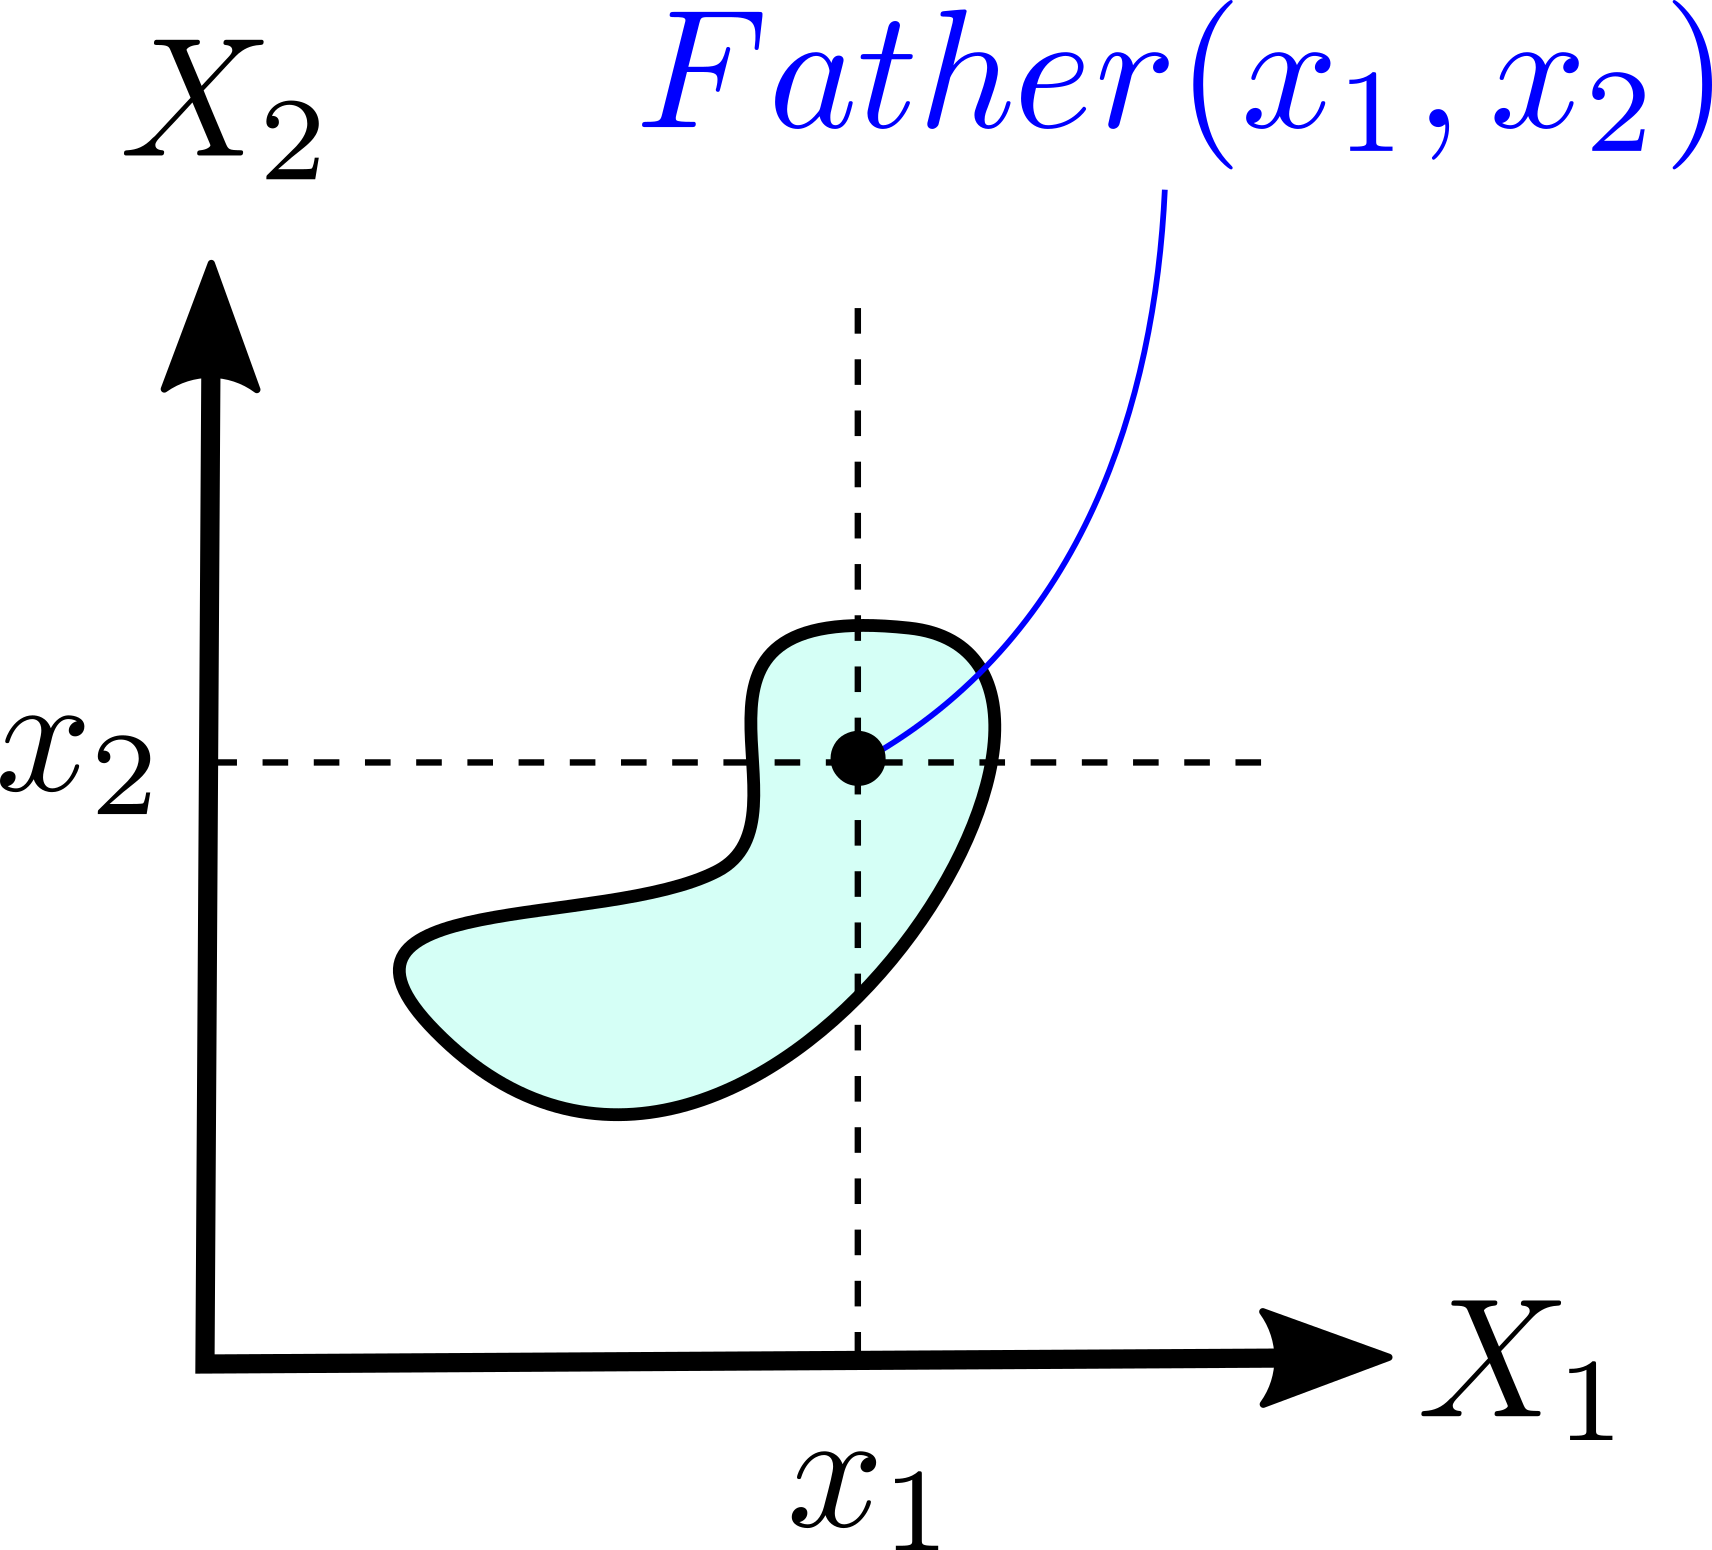
\includegraphics[scale=0.5]{cylindric-relation.png}}}
\quad \quad \quad
\vcenter{\hbox{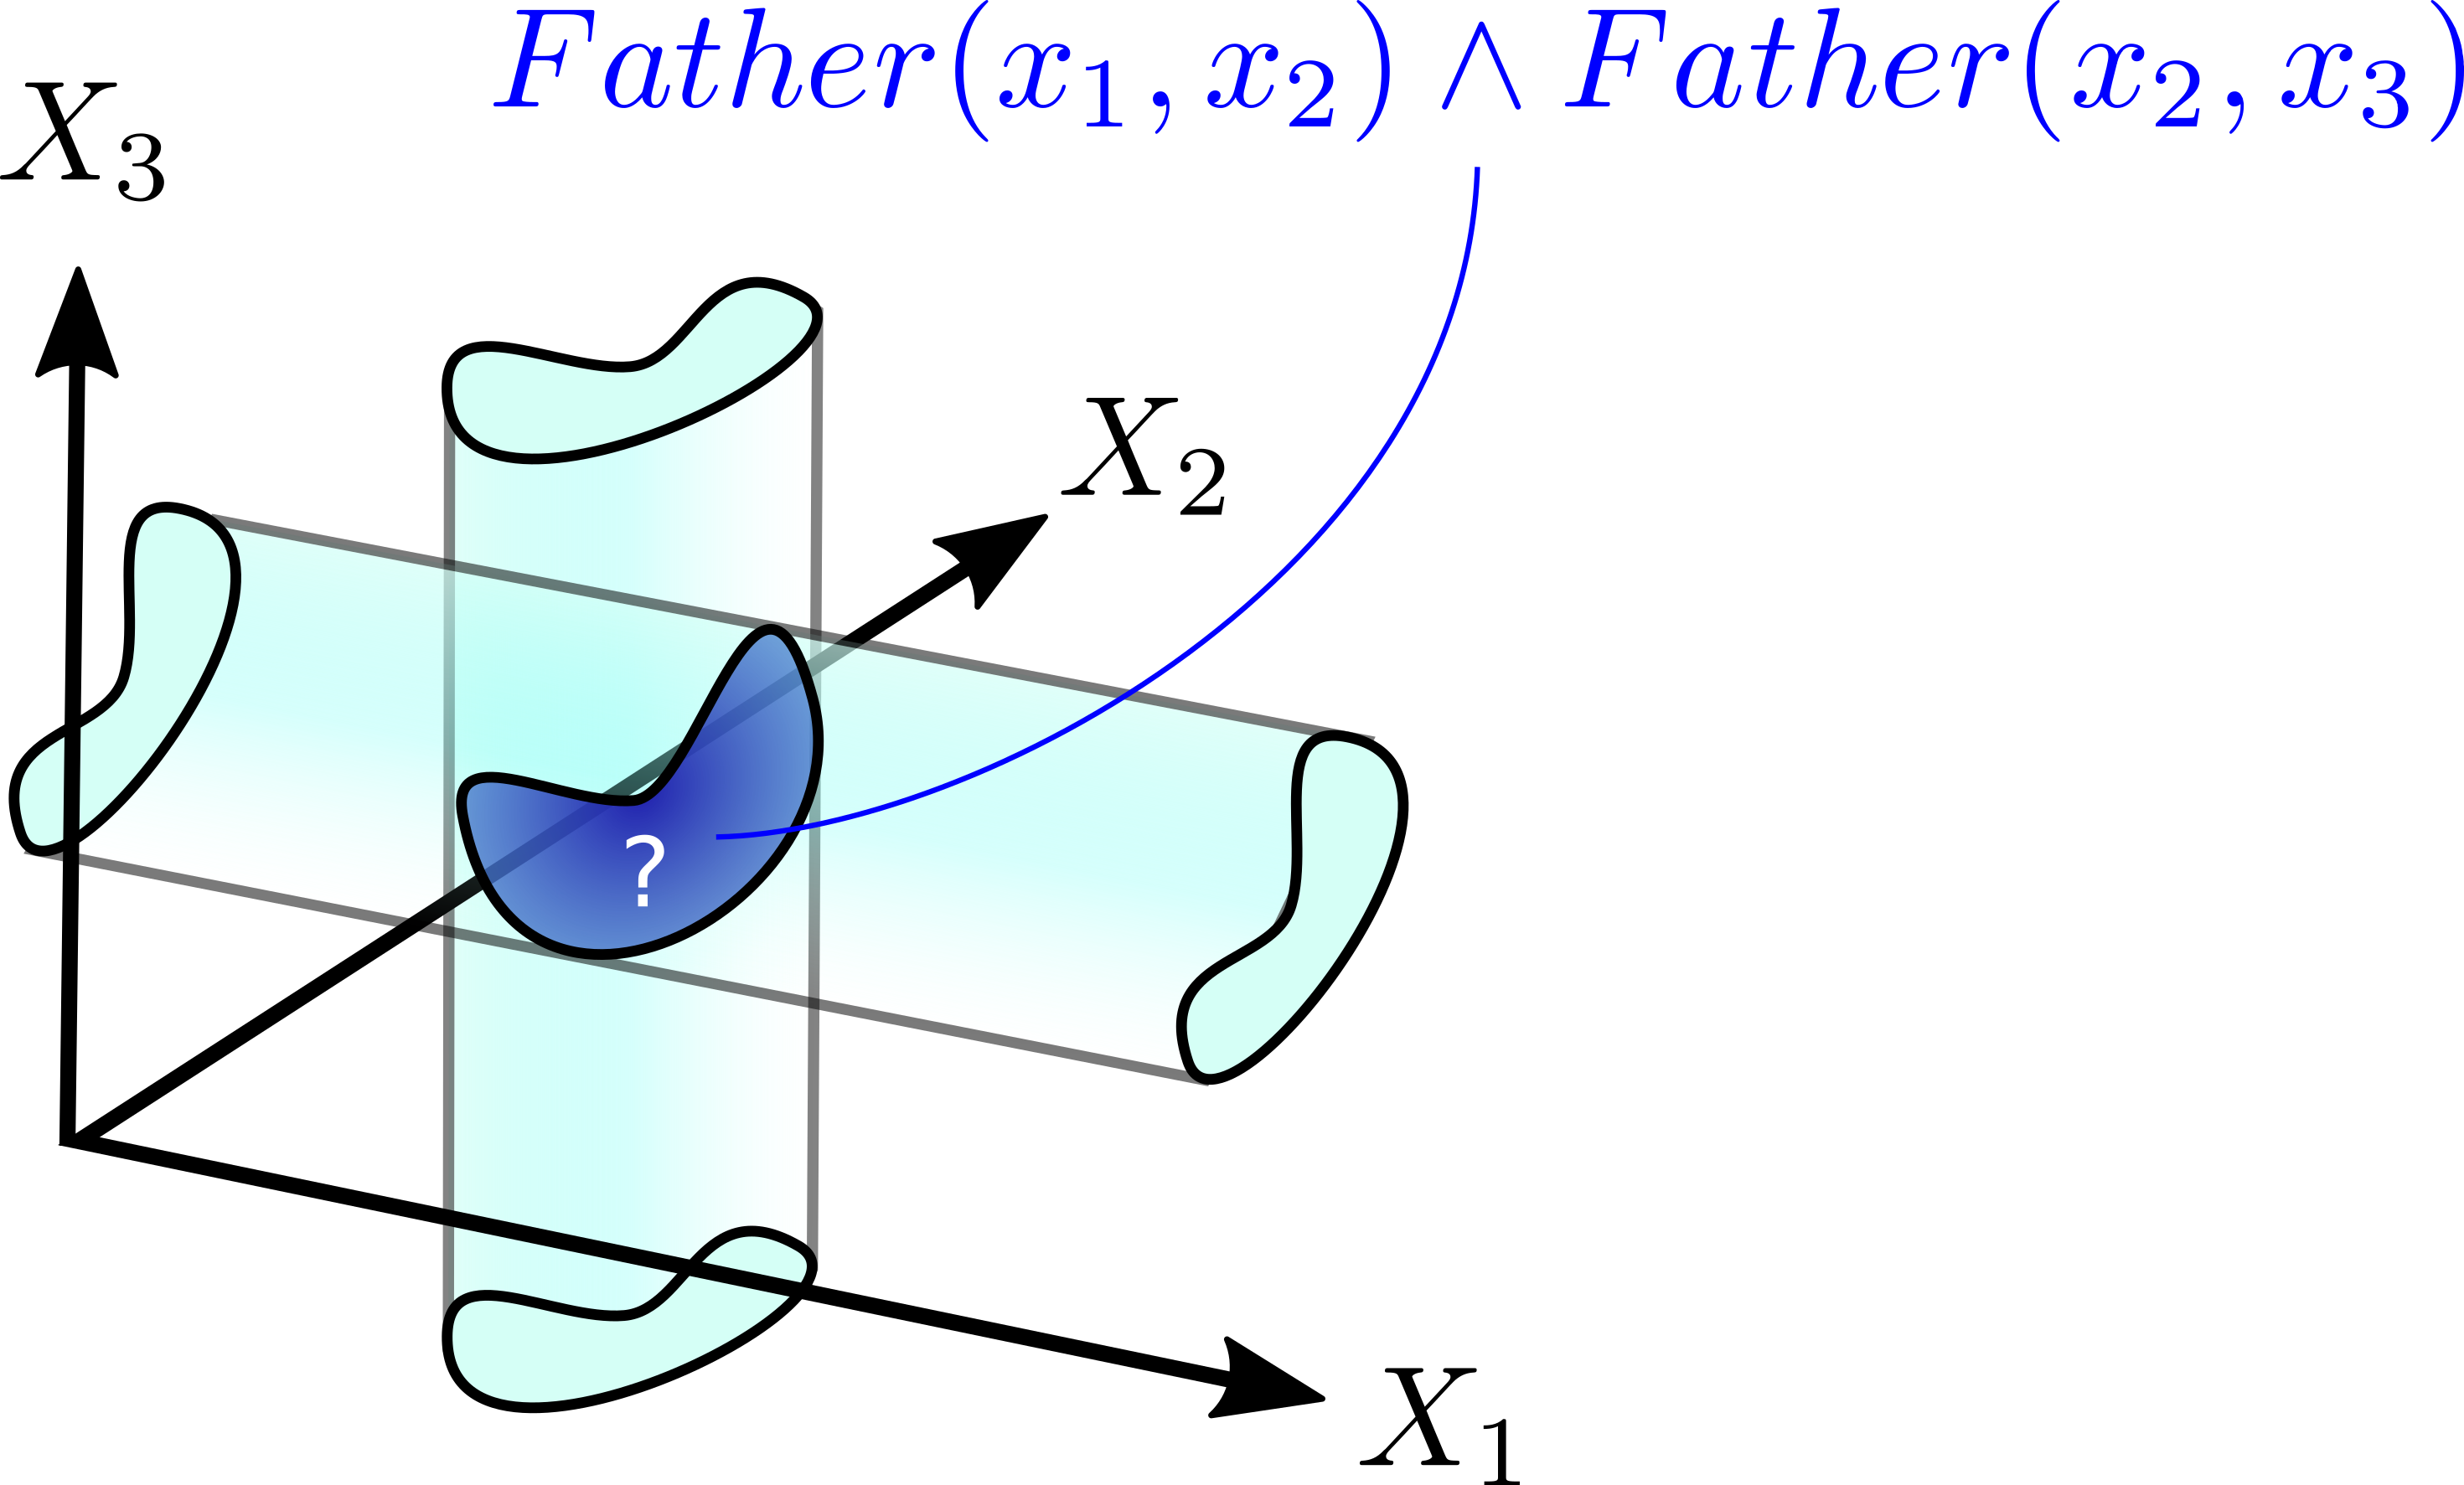
\includegraphics[scale=0.5]{cylindric-relation-intersection.png}}}
\end{equation}
And ``linkages'' cause the graph of the $\vdash$ map to \textit{pass through} diagonal lines such as follows:
\begin{equation}
\label{eqn:diagonal-shapes}
\vcenter{\hbox{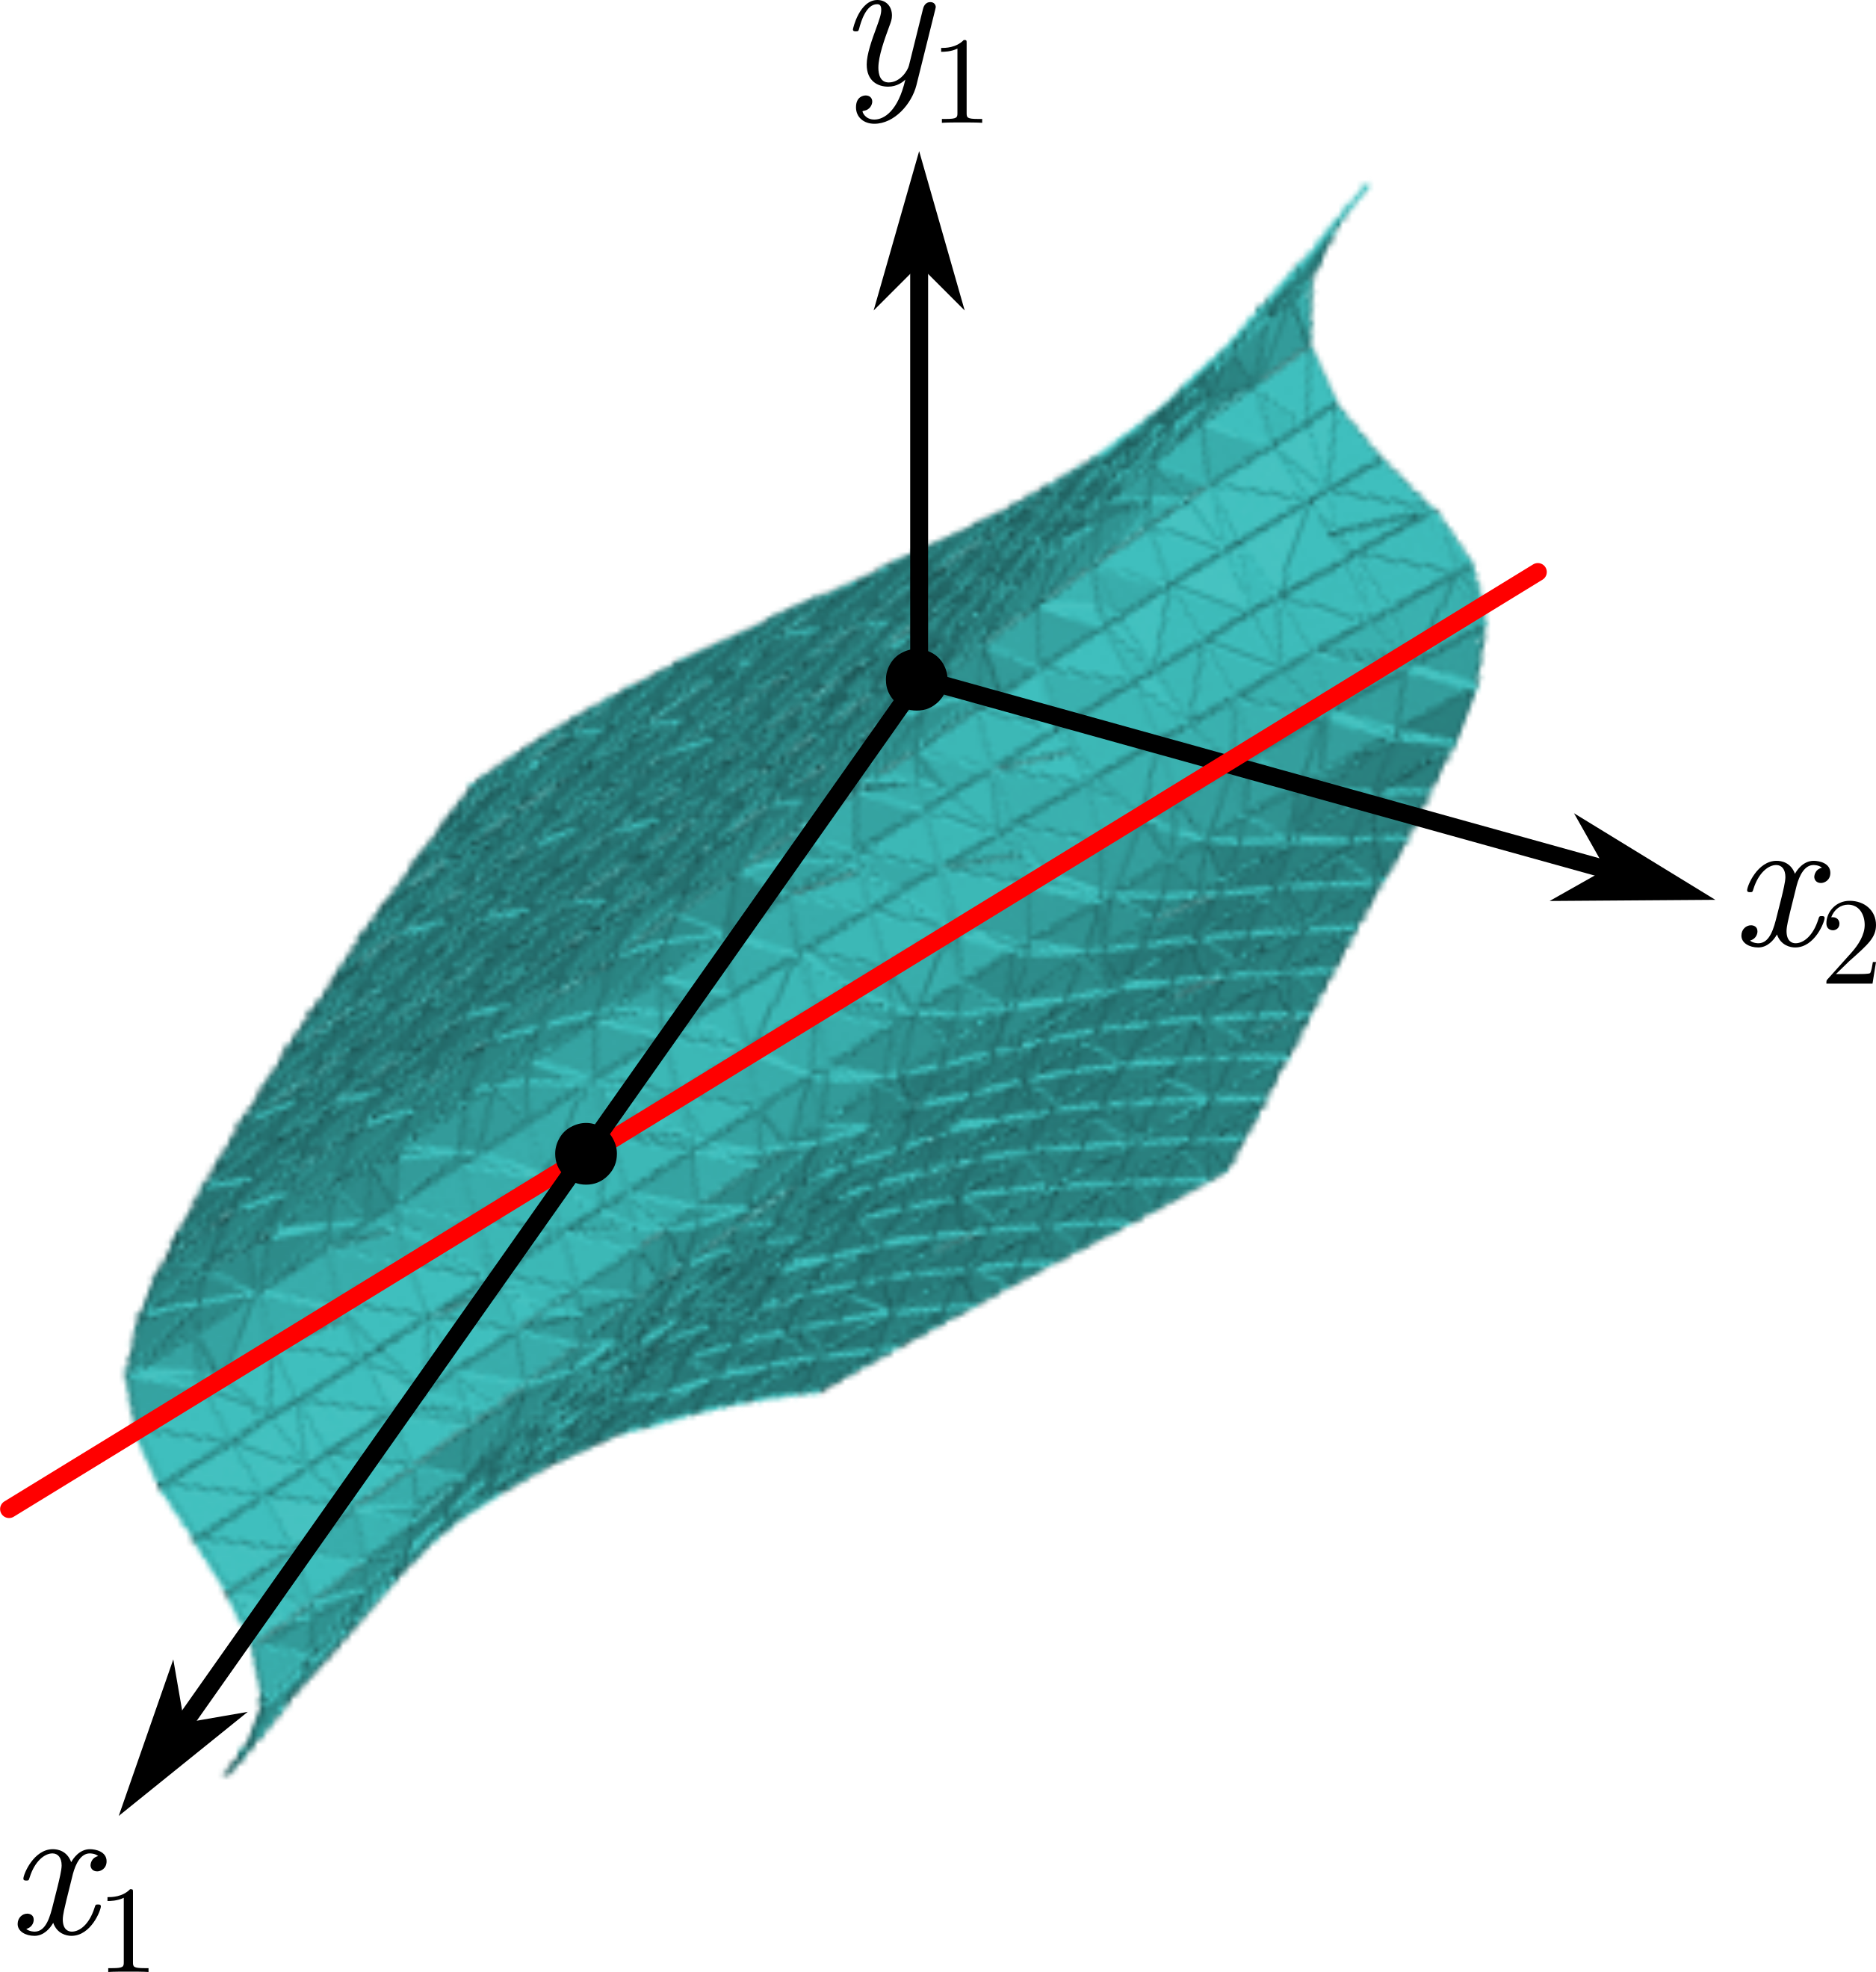
\includegraphics[scale=0.3]{diagonal.png}}}
\end{equation}
We are trying to use neural networks to approximate such functions (\textit{ie}, these geometric shapes).  One can visualize, as the shape of neural decision-boundaries approximate such diagonals, \uline{the matching of first-order objects gradually go from partial to fully-quantified} $\forall$ and $\exists$.  This may be even better than if we fix the logic to have exact quantifications, as quantified rules can be learned gradually.  %Since NNs are universal function approximators, they can in principle achieve that. 
There is also \textit{empirical} evidence that NNs can well-approximate logical maps, because the \textit{symbolic} matching and substitution of logic variables is very similar to what occurs in \textit{machine translation} between natural languages;  In recent years, deep learning is fairly successful at the latter task.

\subsection{Form of a logic rule}

So what exactly is the logic structure? Recall that inside our RL model:
\begin{itemize}
	\item state $\vect{x} \in \mathbb{X}$ = mental state = set of logic propositions $\mathsf{P}_i \in \mathbb{P}$
	\item environment = state space $\mathbb{X}$ = mental space
	\item actions $\vect{a} \in \mathbb{A}$ = logic rules
\end{itemize}

For our current prototype system, an action = a logic \textbf{rule} is of the form:
\newcommand{\Atom}{\,\mathsf{C}}
\renewcommand{\!}{\mkern6mu}
\begin{equation}
\label{eqn:logic-rule}
\overbrace{ \Atom^1_1 \Atom^1_2 \Atom^1_3 \! \wedge \! \underbrace{\Atom^2_1 \Atom^2_2 \Atom^2_3}_{\makebox[0pt]{each literal made of $m$ atomic concepts, $m = 3$ here}}  \! \wedge \! .... \! \wedge \! \Atom^k_1 \Atom^k_2 \Atom^k_3}^{\mbox{conjunction of $k$ literal propositions}} \quad \Rightarrow \quad \overbrace{ \Atom^0_1 \Atom^0_2 \Atom^0_3 }^{\mbox{conclusion}}
\end{equation}
where a \textbf{concept} can be roughly understood as a \textbf{word vector} as in Word2Vec \cite{Word2Vec}.  Each $\Atom \in \mathbb{R}^d$ where $d$ is the dimension needed to represent a single word vector or concept.

We use a ``free'' neural network (\textit{ie}, standard feed-forward NN) to approximate the set of \textit{all} rules.  The \textbf{input} of the NN would be the state vector $\vect{x}$:
\begin{equation}
\Atom^1_1 \Atom^1_2 \Atom^1_3 \! \wedge \! \Atom^2_1 \Atom^2_2 \Atom^2_3 \! \wedge \! .... \! \wedge \! \Atom^k_1 \Atom^k_2 \Atom^k_3 .
\end{equation}
We fix the number of conjunctions to be $k$, with the assumption that conjunctions of length $< k$ could be filled with ``dummy'' (always-true) propositions.

The \textbf{output} of the NN would be the conditional \textbf{probability} of an action:
\begin{equation}
P(\mbox{action } | \mbox{ state}) := \pi(\Atom_1 \Atom_2 \Atom_3 \; | \; \vect{x}).
\end{equation}
Note that we don't just want the action itself, we need the \textbf{probabilities} of firing these actions.  The \textbf{Bellman update} of reinforcement learning should update the conditional probabilities over such actions (\S\ref{sec:Gaussian-kernels}).

%\section{Implementation issues}

% Mathematically, a \textbf{neural network} is a non-linear function with many parameters (called ``weights'', organized as layers of matrices):
%\begin{eqnarray}
%\mbox{\footnotesize each layer's } \tikzmark{ww} \mbox{\footnotesize \textbf{weight} matrix} \quad \quad \mbox{\footnotesize total \# of layers} \tikzmark{LL} \nonumber \\
%\nonumber \\
%\vect{F}(\vect{x}) = \sigmoid(W_1 \tikzmark{wa} \sigmoid(W_2 \tikzmark{wb} ... \sigmoid( W_L \tikzmark{wc} \tikzmark{L} \; \vect{x} )))
%\begin{tikzpicture}[overlay,remember picture]
%\draw[-, shorten <=26pt, transform canvas={shift={(-10pt,10pt)}}] (ww.center) to (wa.center);
%\draw[-, shorten <=38pt, transform canvas={shift={(-10pt,10pt)}}] (ww.center) to (wb.center);
%\draw[-, shorten <=46pt, transform canvas={shift={(-10pt,10pt)}}] (ww.center) to (wc.center);
%\draw (LL.center) +(-15pt,-3pt) -- ([shift={(-2pt,6pt)}]L.center);
%\end{tikzpicture}
%\end{eqnarray}
%where $\sigmoid$ is a sigmoid-shaped non-linear function, applied component-wise to the vectors.

\subsection{Structure of a logic-based AI system}
\label{sec:LBAI-structure}

Besides the intrinsic structure of a logic, the AI system has a structure in the sense that it must perform the following operations iteratively, in an endless loop:
\begin{equation}
\vcenter{\hbox{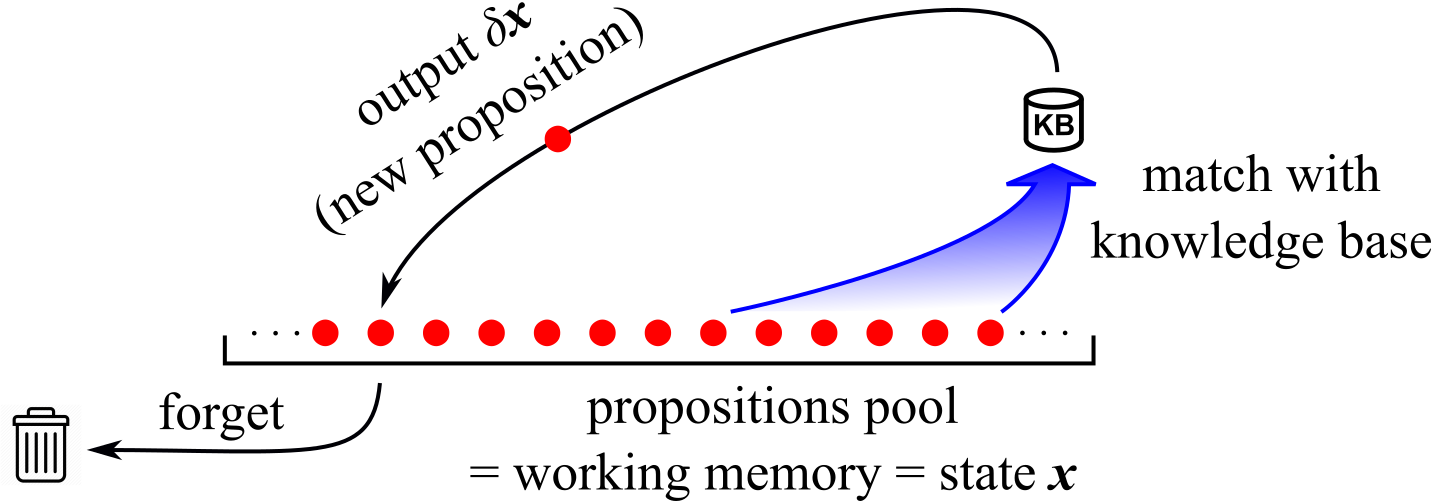
\includegraphics[scale=0.5]{classical-AI-architecture.png}}}
\label{fig:LBAI}
\end{equation}
\begin{itemize}
	\item \textbf{Matching} --- the $\KB$ of rules is matched against the current state $\vect{x}$, resulting in a (stochastically selected, \textit{eg} based on $\epsilon$-greedy) rule:
		\begin{eqnarray}
		\boxed{\mbox{Match}} \quad
		( \vect{x} \stackrel{?}{=} \KB ) \;: \mathbb{X} &\rightarrow& ( \mathbb{X} \rightarrow \mathbb{P} ) \nonumber \\
		\label{eqn:matching}
		\vect{x} &\mapsto& \vect{r} 
		\end{eqnarray}
	--- In categorical logic, matching is seen as finding the \textbf{co-equalizer} of 2 terms which returns a \textbf{substitution} \cite{Goguen1989} \cite{Lawvere1963} \cite{Lawvere2003} \cite{Jacobs1999}.  The substitution is implicit in our formulation and would be \textit{absorbed} into the neural network in our architecture.  \\
	--- Matching should be performed over the entire \textbf{working memory} = the state $\vect{x}$ which contains $k$ literals.  This is combinatorially time-consuming.  The celebrated \textbf{\textit{Rete}} algorithm \cite{Rete-algorithm} turns the set of rules into a tree-like structure which is efficient for solving (\ref{eqn:matching}).
	\item \textbf{Rule application} --- the rule is applied to the current state $\vect{x}$ to produce a new literal proposition $\delta \vect{x}$:
		\begin{eqnarray}
		\boxed{\mbox{Apply}} \quad
		\vect{r} : \mathbb{X} &\rightarrow& \mathbb{P} \nonumber \\
		\vect{x} &\mapsto& \vect{r}(\vect{x}) = \delta \vect{x}
		\end{eqnarray}
	\item \textbf{State update} --- the state $\vect{x}$ is \textit{destructively} updated where one literal $\mathsf{P}_j \in \vect{x}$ at the $j$-th position is \textbf{forgotten} (based on some measure of attention / interestingness) and over-written with $\delta \vect{x}$:
		\begin{equation}
		\boxed{\mbox{Update}} \quad
		\vect{x} = (\mathsf{P}_1, \mathsf{P}_2, ..., \mathsf{P}_j, ..., \mathsf{P}_k ) \mapsto (\mathsf{P}_1, \mathsf{P}_2, ..., \delta \vect{x}, ..., \mathsf{P}_k )
		\end{equation}
\end{itemize}
All these operations are represented by functions parametrized by some variables $\Theta$ and they must be made \textit{differentiable} for gradient descent.

\begin{comment}

\subsection{Topological / metric structure of the domain $\mathbb{X}$}

In order to apply reinforcement learning, we need to calculate the gradient $\displaystyle \nabla_{\Theta} V(\vect{x}(t))$.  For this, the domain $\mathbb{X}$ needs to have some kind of differentiable structure.  So we proceed as follows:
\begin{itemize}
	\item Time steps are discrete.  Using continuous time increases the computational burden seemingly without any benefits.
	\item Atomic concepts $\mathsf{C}$'s are embedded in a vector space, thanks to the technique of \textbf{Word2Vec} \cite{Word2Vec}.  We assume that such a ``concept embedding'' is sensible without further explaining its justification.
	\item Propositions $\mathsf{P} \in \mathbb{P}$ are composed of atomic concepts, hence they are also embeddable in vector space.
	\item The state $\vect{x} \in \mathbb{X}$ is a set (seen as a list) of propositions, thus also inherits a vector-space embedding.
	\item However, it is well-known that \textbf{syntactic} distance can be very different from \textbf{semantic} distance (sentences that appear similar may differ drastically in meaning).  From the point of view of logic, the 2 metrics \uline{must not be confused}.
	\item It is also well-known that the semantic distance (ie, how many logic steps are required to deduce one logic state from another) is related to \textbf{Kolmogorov complexity} \cite{Li2008} and is \textit{incomputable}, which however can be \textit{approximated}.  It is my belief that all AGI systems must approximate this metric in one way or another.
	\item For each time step, the state $\vect{x}$ should move by one logic rule $\vect{u} \equiv \dot{\vect{x}}$; If a proposition has merely moved via syntactic similarity, this is not considered ``genuine'' movement in the dynamical / control theoretic sense.  Each logic step is $1$ unit of semantic distance.
	\item In our architecture, logic rules are parametrized by $\Theta \in \mathbb{R}^N$ which are the weights of a neural network $\vect{F}$.  Thus, rules exist in a \textbf{continuum}.  
	\item The output of a rule is a new proposition $\delta \vect{x} \in \mathbb{P}$ which is also embedded in vector space.
	\item Therefore, at each time step, a point $\vect{x}$ in state space $\mathbb{X}$ is only allowed to move \textit{via} the continuum of rules parametrized by $\Theta \in \bbTheta$, which is different from the neighborhood of $\vect{x}$ based on similarity:
	\begin{equation}
	\vcenter{\hbox{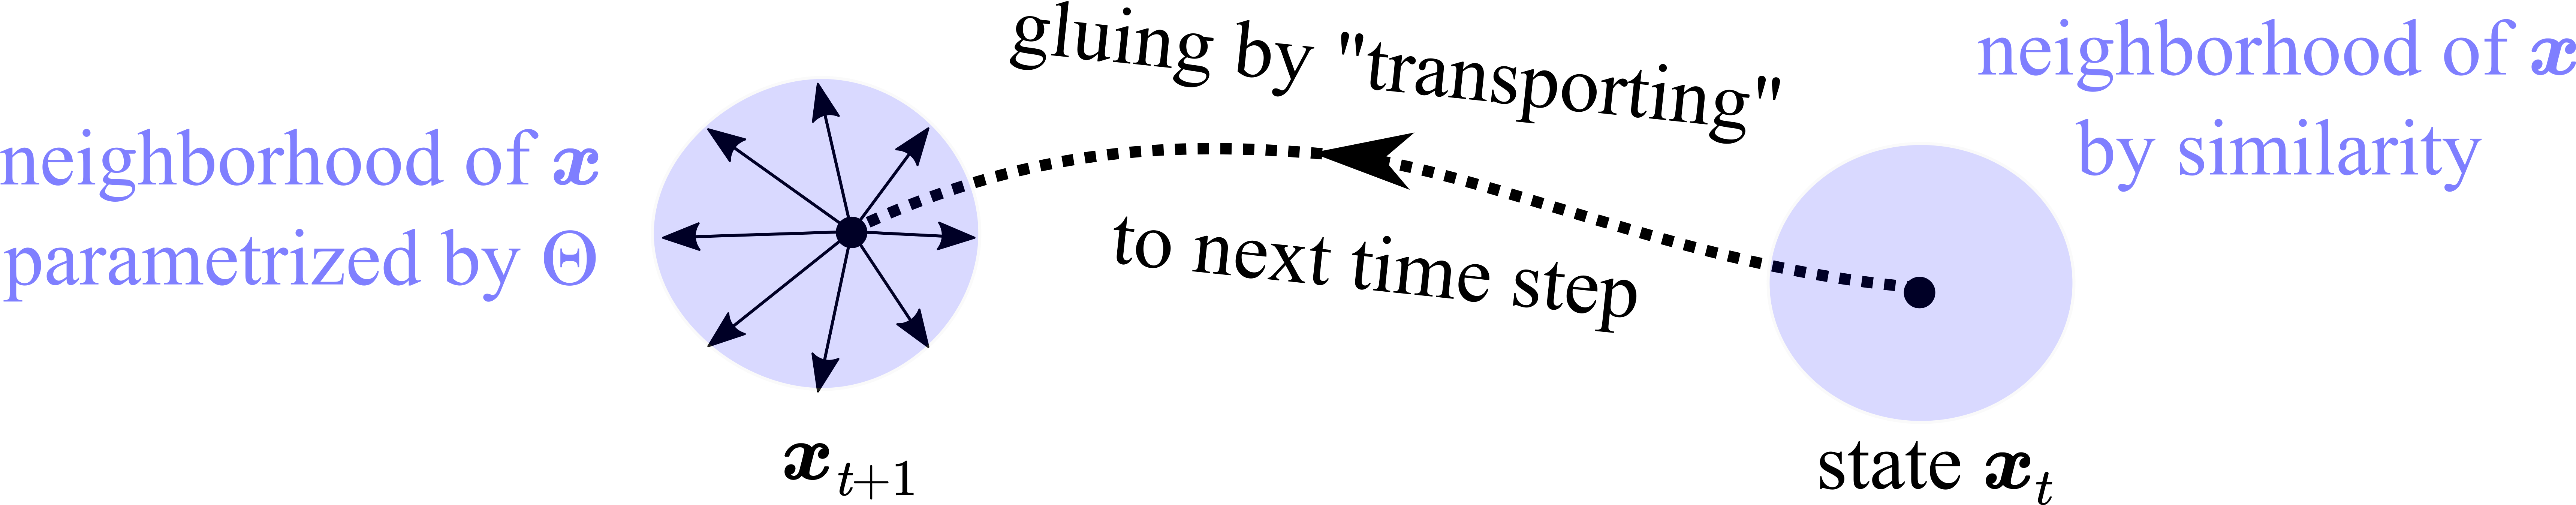
\includegraphics[scale=0.5]{gluing-by-teleportation.png}}}
	\end{equation}
	(Now the neighborhood of $\vect{x}_{t+1}$ is a subset $\subset \bbTheta$ which replaces $\mathbb{X}$)
	\item In short, what we have here is \uline{discrete-time dynamics occurring in continuous space}.
	\item The objective function $J$ rewards correct answers while penalizing logic path lengths, thus forcing the system to acquire intelligence. This knowledge is represented in the function $\vect{F}$ parametrized by $\Theta$.  It is intuitively obvious that $\vect{F}$ contains an implicit approximation of Kolmogorov complexity.
\end{itemize}

\end{comment}


\subsection{Commutativity of logic conjunctions}
% \label{sec:commutative-structure}

One basic characteristic of (classical) logic is that the conjuction $\wedge$ is \textbf{commutative}:
\begin{equation}
\mathsf{P} \wedge \mathsf{Q} \quad \Leftrightarrow \quad \mathsf{Q} \wedge \mathsf{P} .
\end{equation}
This restriction may significantly reduce the size of the search space.  If we use a neural network to model the deduction operator $\vdash: \mathbb{P}^k \rightarrow \mathbb{P}$, where $\mathbb{P}$ is the space of literal propositions, then this function should be \textbf{symmetric} in its input arguments.

I have considered a few solutions to this problem, including an algebraic trick to build ``symmetric'' neural networks (but it suffers from combinatorial inefficiency), and using Fourier transform to get a ``spectral'' representation of the state, which remained rather vague and did not materialize.

As of this writing
\footnote{Convolutional NNs are only \textit{translation}-invariant.  The Transformer \cite{Vaswani2017} architecture is \textit{equivariant} under permutations (meaning permuted inputs give permuted outputs), but it implicitly contains a recurrence similar to ours.}
I have settled on the ``carousel'' solution:  All the propositions in working memory will enter into a loop, and the reasoning operator \uline{acts on a hidden state $\vect{H} = {\color{green}\bullet}$ and one proposition $\mathsf{P}_i = {\color{red}\bullet}$ at a time}:
\begin{equation}
\label{fig:carousel}
\vcenter{\hbox{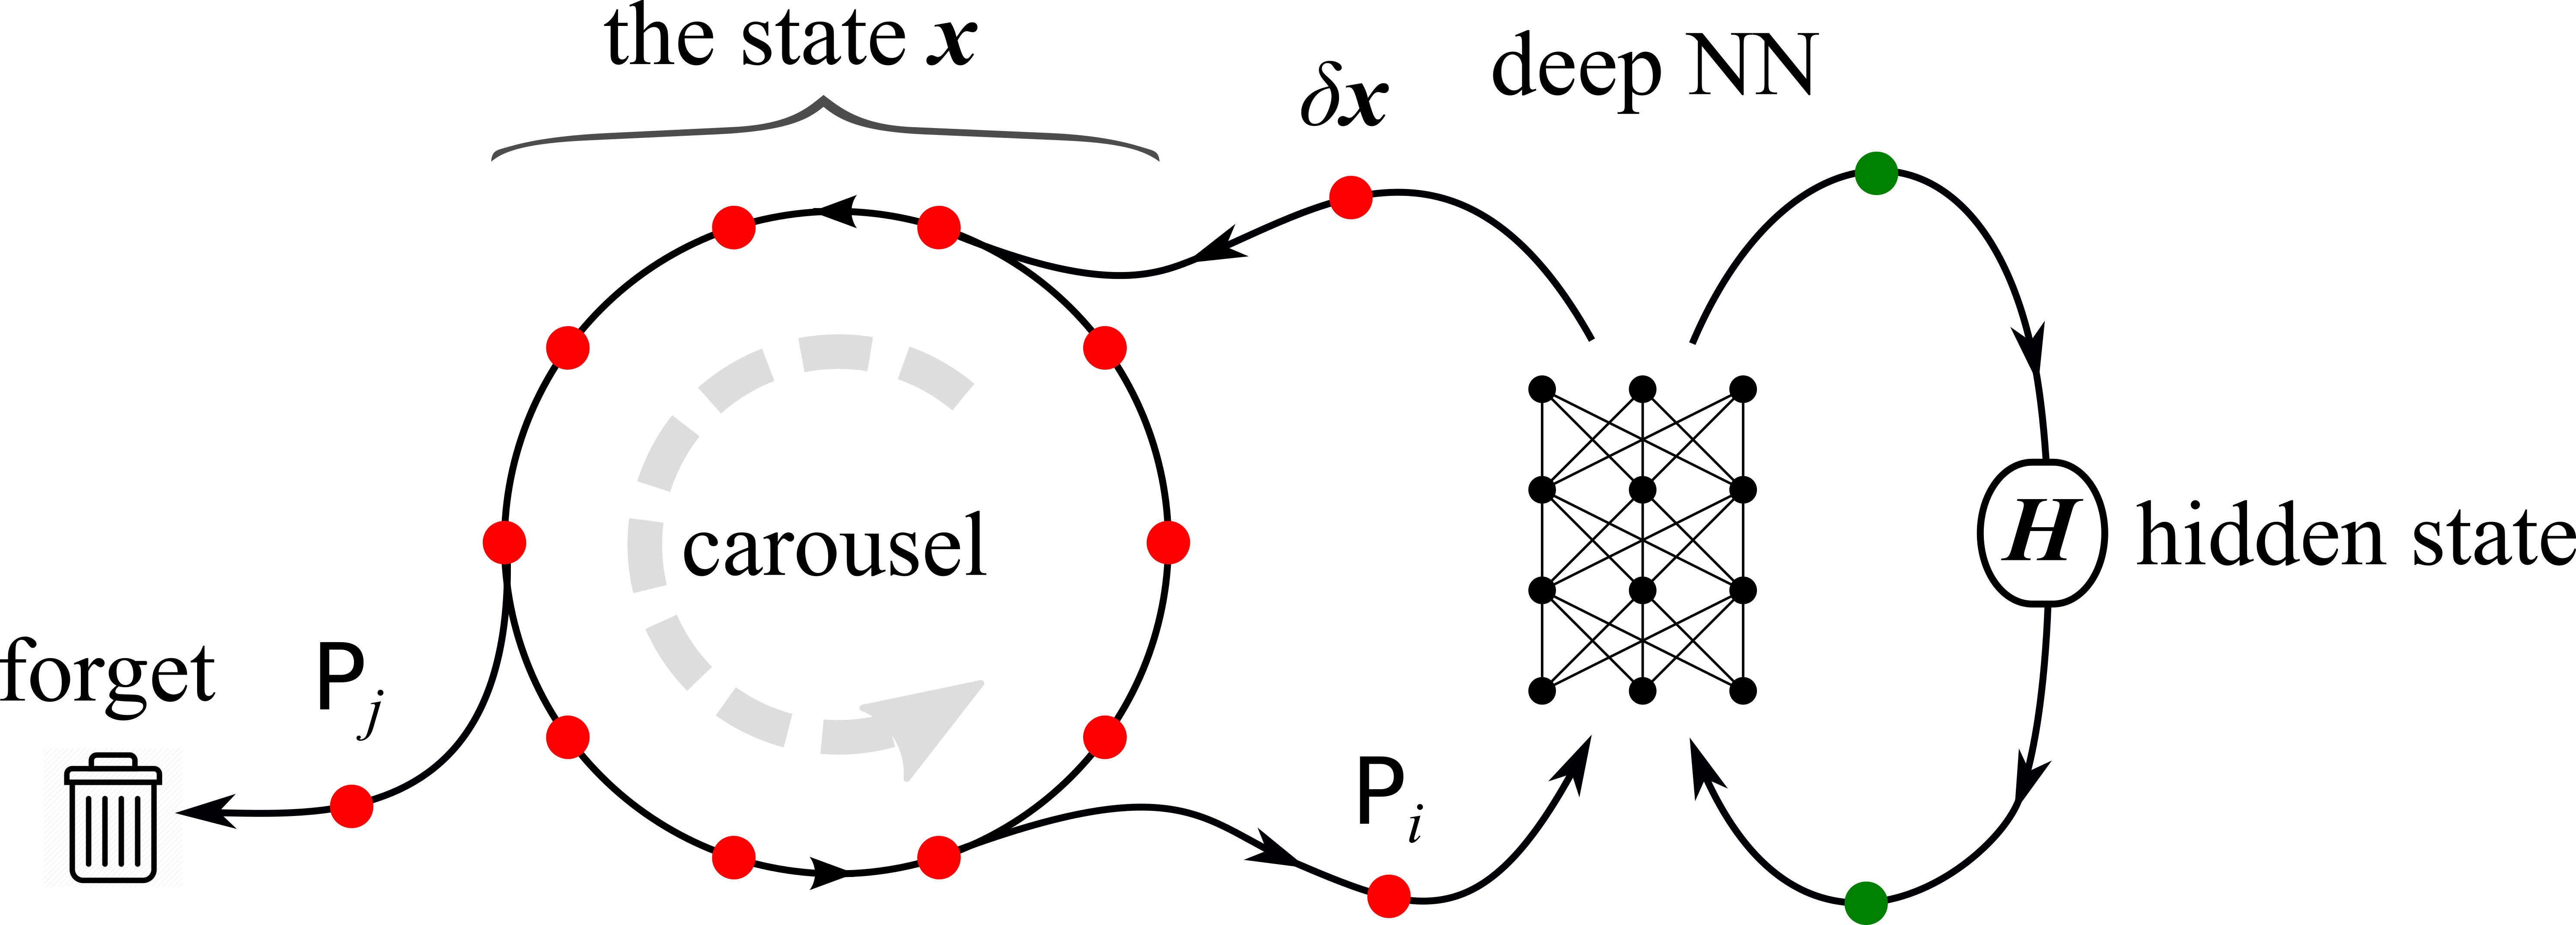
\includegraphics[scale=0.5]{carousel.png}}}
\end{equation}

Notice that the working memory $\vect{x}$ is itself a hidden state, so $\vect{H}$ can be regarded as a \textit{second-order} hidden state.

This architecture has the advantage of being simple and may be biologically plausible (the human brain's working memory).  

I believe in the maxim: \textit{Whatever can be done in time can be done in space}.  The diagram (\ref{fig:carousel}), when unfolded in time, can be expressed in this functional form:
\begin{equation}
\vect{F}_{\mathrm{sym}}(\mathsf{P}_0, ..., \mathsf{P}_k) = \vect{f}(\mathsf{P}_k, \vect{f}(\mathsf{P}_{k-1}, \vect{f}(..., \vect{f}(\mathsf{P}_0, \vec{\emptyset})))) .
\end{equation}
%It may be possible to solve the functional equation to eliminate the recurrent structure.   
$\vect{F}_{\mathrm{sym}}$ means that the function is invariant under the action of the symmetric group $\mathfrak{S}_k$ over propositions.  Such symmetric NNs have been proposed in \cite{Gens2014} \cite{Bie2019} \cite{Ravanbakhsh2016} \cite{Ravanbakhsh2017} \cite{Qi2016} \cite{Qi2017} \cite{Zaheer2017}.

\begin{comment}
A simple fact:  If $\vect{F}(\vect{p},\vect{q})$ is any function, then
\begin{equation}
\vect{F}(\vect{p},\vect{q}) + \vect{F}(\vect{q},\vect{p}) \quad \mbox{or} \quad \vect{F}(\vect{p},\vect{q})  \vect{F}(\vect{q},\vect{p})
\end{equation}
would be symmetric functions in $(\vect{p},\vect{q})$.  This can be easily extended to $\mathbb{P}^k$.  % We will use the additive method.

Thus if $\vect{F}$ is a ``free'' neural network, we can create a symmetric NN (via addition):
\begin{equation}
\vect{F}_{\mathrm{sym}}(\vect{x}) = \frac{1}{k!} \sum_{\sigma \in \mathfrak{S}_k} \vect{F}(\sigma \cdot \vect{x})
\end{equation}
where $\mathfrak{S}_k$ is the symmetric group of $k$ elements, and $\vect{x} = \vect{p}_1 \wedge \vect{p}_2 \wedge ... \vect{p}_k$.  Back-propagation can be easily adapted to such symmetric NNs.  However, if $K$ is the size of working memory, it would require to perform forward propagation $k! \;_K C_k = \;_K P_k$ times for each step, which is computationally inefficient (the same reason why \textit{Rete} was needed in classical AI).

So we would not use this idea, but it is illustrative of the problem.

\subsection{Spectral representation of states}

Now consider another simple idea.  Suppose we have 3 vectors $(\vect{v}_1, \vect{v}_2, \vect{v}_3)$ in a 1-dimensional vector space $V$, and we attach a \textbf{truth value} $\top = 1$ to each vector.  Then we try to approximate the \textbf{graph} of truth values $\top(\vect{v})$ as a ``wave'' using Fourier or wavelet transform:
\begin{equation}
\vcenter{\hbox{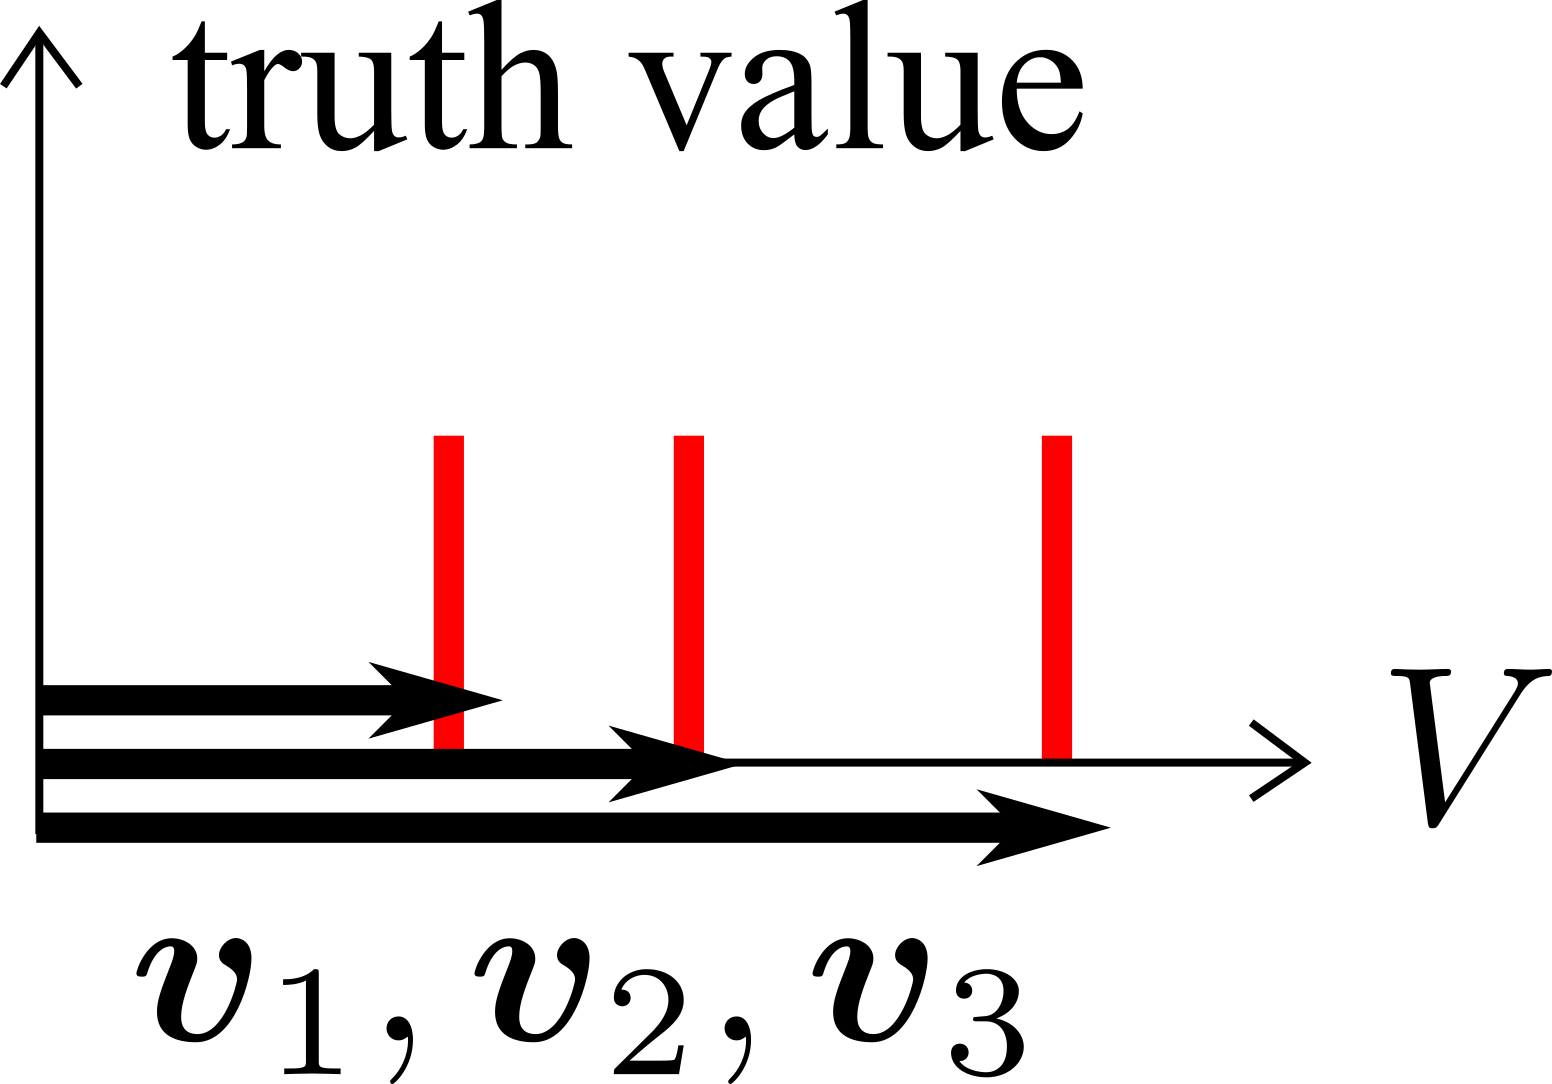
\includegraphics[scale=0.6]{Fourier-representation-0.png}}}
\quad \Rightarrow \quad
\vcenter{\hbox{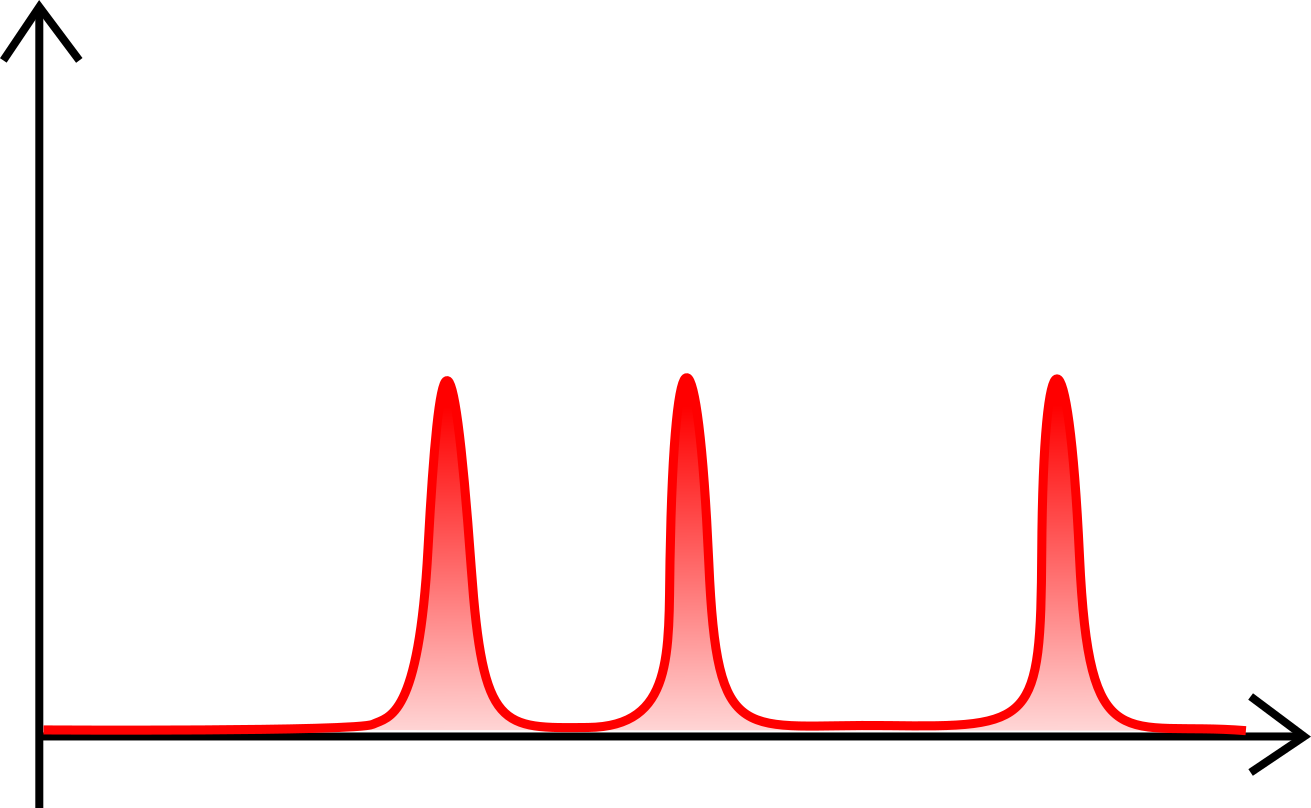
\includegraphics[scale=0.6]{Fourier-representation-0B.png}}}
\end{equation}

The resulting representation has some nice properties:
\begin{itemize}
	\item If we permute $(\vect{v}_1, \vect{v}_2, \vect{v}_3)$, the graph (and thus its spectrum) remains the same, \textit{ie}, the representation is \uline{invariant under permutations}
	\item We can add more vectors to the graph without changing the size of the spectral representation, \textit{ie}, it is relatively insensitive to the number of vectors
\end{itemize}

We can extend this idea to the \textbf{multi-dimensional} case where the literal proposition vector $\vect{p} \in \mathbb{P} = \mathbb{R}^{3d}$ 
\footnote{For example, a typical $d$ from Word2Vec or GloVe is 200, so $3d = 600$.}
and the state $\vect{x}$ consists of $k$ vectors $= \vect{p}_1 \wedge \vect{p}_2 \wedge ... \vect{p}_k$.  In other words, we need to apply Fourier transform to a wave over $3d$ dimensions.  Moreover, we can have truth values in the range $[-1,1]$, which can be construed as \textbf{fuzzy} truth values, or in the range $[0,1]$, regarded as the probability of \textbf{stochastic actions} (as is common in policy-gradient methods).
\begin{equation}
% \begin{tabular}{ccc}
% proposition vectors in $n$-dim space & & wave over $n$-dim space \\
% with {\color{red}truth values} \vspace*{0.5em} & & \\
\vcenter{\hbox{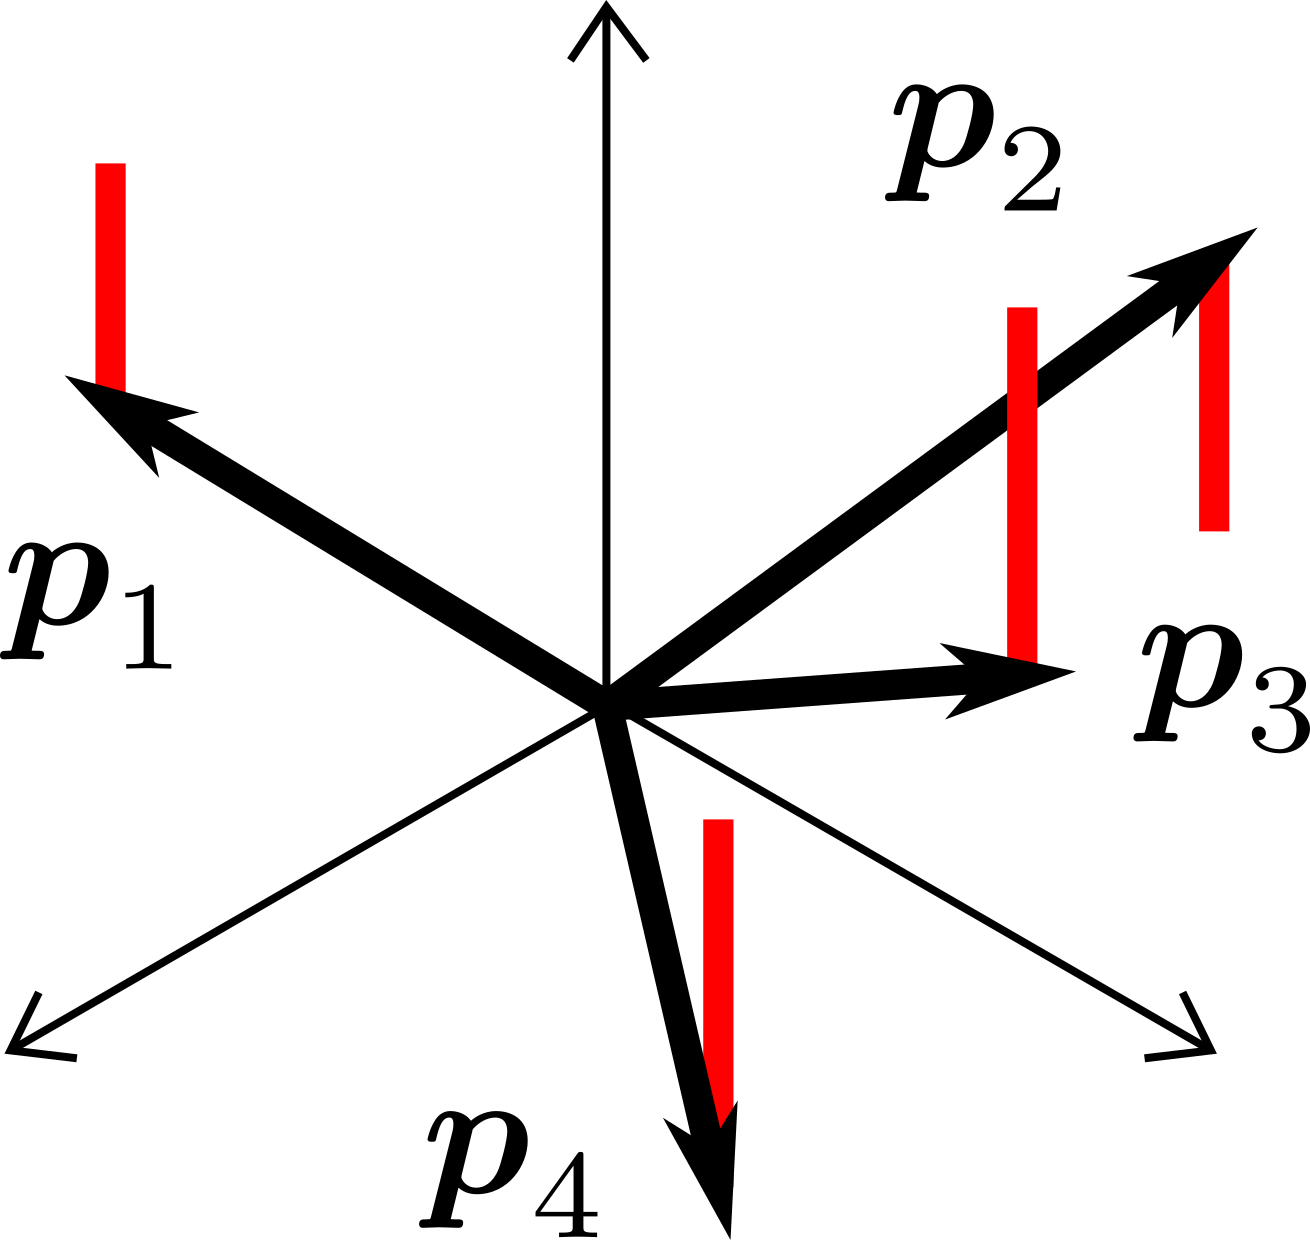
\includegraphics[scale=0.6]{Fourier-representation-1.png}}} 
\quad \Rightarrow \quad
\vcenter{\hbox{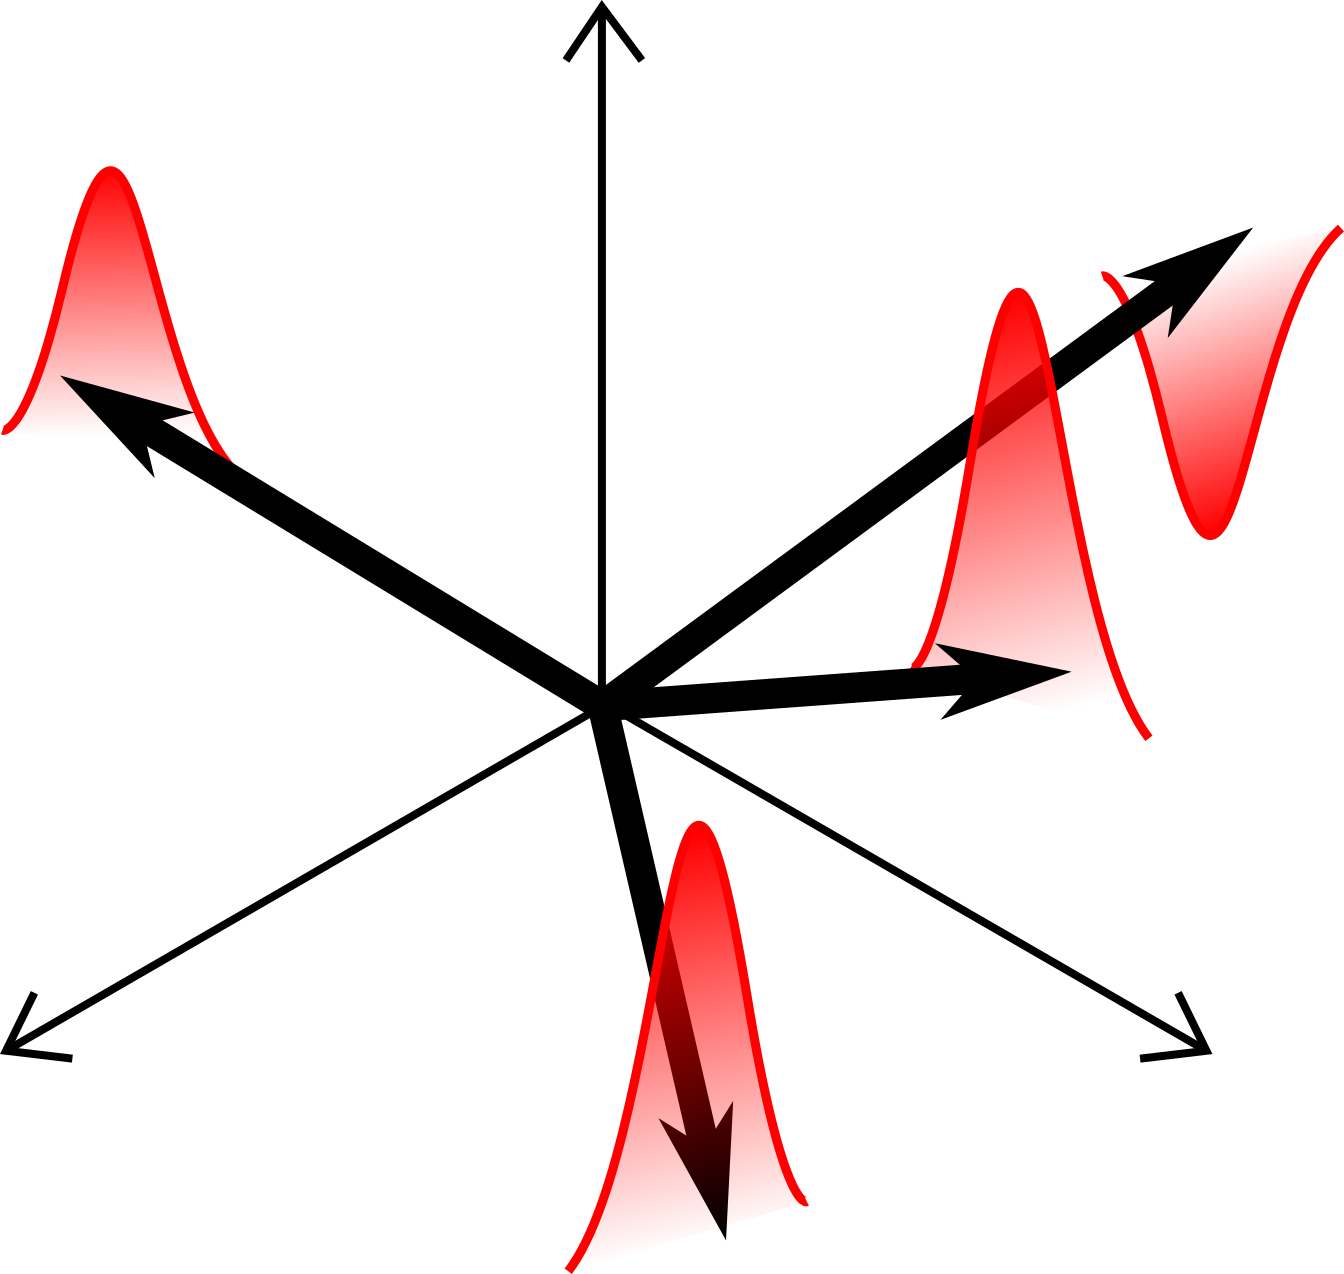
\includegraphics[scale=0.6]{Fourier-representation-2.png}}} 
% \end{tabular}
\end{equation}

Notice that our NN would \textit{input} from the spectral representation and \textit{output} the normal representation.

With this approach, the geometric shapes of (\ref{eqn:cylindric-shapes}) and (\ref{eqn:diagonal-shapes}) would be distorted in very complicated ways.  It remains to be verified whether NNs can learn this task effectively.
\end{comment}

\subsection{Logic actions}
\label{sec:logic-actions}

The output of a logic rule is a proposition $\delta \vect{x} \in \mathbb{P}$, the space of propositions.  This is a continuous space (due to the use of Word2Vec embeddings).

From the perspective of reinforcement learning, we are performing an action $\vect{a}$ (the logic rule) from the current state $\vect{x}$.  The neural network in (\ref{fig:carousel}) is a parametrized function $\vect{F}_{\Theta}$ that accepts $\vect{x}$ and outputs $\delta \vect{x}$.  We want to \textbf{gradient-descent} on $\Theta$ to get the optimal set of actions, ie, a \textbf{policy}.

To solve the RL problem, 2 main options are: \textbf{value-iteration} (\textit{eg} Q-learning) and \textbf{policy-iteration}.

In \textbf{Q-learning}, we try to learn the action-value function $Q(\vect{a}|\vect{x}) \rightarrow \mathbb{R}$.  The policy is obtained by choosing $\displaystyle \arg \max_{\vect{a}} Q(\vect{a}|\vect{x})$ at each step.  In our logic setting, the action space $\mathbb{A} \ni \vect{a}$ is continuous.  As is well known, if we use an NN to represent $Q(\vect{a}|\vect{x})$, the evaluation of $\displaystyle \arg \max_{\vect{a}}$ would be rather awkward, which is why $Q$-learning is widely seen as ill-suited for continuous actions.

It is much easier for the NN to directly output (a fixed number of) stochastic actions, thus avoiding the \textit{curse of dimensionality}.  Such a function is a \textbf{stochastic policy} $\pi(\vect{a}|\vect{x})$.

%All the ``knowledge'' of our agent would be contained in the policy function $\pi$:
%\begin{eqnarray}
%\pi: \mathbb{X} \times \mathbb{A} &\rightarrow& [0,1] \in \mathbb{R} \nonumber \\
%(\vect{x},\vect{a}) &\mapsto& P(\vect{a} \;|\; \vect{x})
%\end{eqnarray}
%where $\mathbb{X}$ = state space, $\mathbb{A}$ = action space, $P(\cdot)$ = conditional probability.

%In reinforcement learning in general, the function space of $\pi$ is of shape:
%\begin{equation}
%\pi : \mathbb{X} \rightarrow \mathbb{R} (\mathbb{A}) = \mathbb{R}^{\mathbb{A}} .
%\end{equation}
%For example, if $\mathbb{A}$ has finitely 10 discrete actions, $\mathbb{R}(\mathbb{A})$ would be $\mathbb{R}^{10}$.  For logic-based agents, $\mathbb{A}$ would be the set of all logic rules, thus very large.  It would be worse if $\mathbb{A}$ is continuously-valued, as we embed propositions in vector space.

In other words, we can use a fixed number of Gaussian kernels (radial basis functions) to approximate the conditional probability distribution of $\pi$ over $\mathbb{A}$.  
%So we may use \textbf{Gaussian kernels} (\textit{ie}, radial basis functions) to approximate $\pi(\vect{a} | \vect{x})$:
%\begin{equation}
%P(\vect{a} | \vect{x}) \approx \hat{P}(\vect{a} | \vect{x}) := \frac{1}{N \sigma} \sum_{i = 1}^{N} \Phi \left( \frac{\vect{a} - \vect{a}_i}{\sigma} \right)
%\end{equation}
%where $\Phi(\vect{\xi})$ is the Gaussian kernel $\frac{1}{\sqrt{2 \pi}} e^{- \vect{\xi}^2 / 2}$. 
For each state $\vect{x}$, our NN outputs a probabilistic \textit{choice} of $c$ actions.  So we only need to maintain $c$ ``peaks'' given by Gaussian kernels.  Each peak is determined by its mean $\delta \vect{x}_i$ and variance $\sigma$.  Both parameters are to be learned.

The size of the FFNN in (\ref{fig:carousel}) seems well within the capacity of current hardware.

\begin{comment}
\subsection{Size of the neural network}

% An action $\vect{a} \in \mathbb{A}$ is a logic rule that takes the state $\vect{x}$ to a proposition $\mathsf{P}$, \textit{ie}, $\mathbb{A} = \mathbb{X} \rightarrow \mathbb{P}$.  
When a rule is applied to a state, it becomes a proposition, so the space of \textit{applied} actions $\mathbb{A}(\vect{x})$ in our case is equivalent to $\mathbb{P}$.

% Also, after our ``Fourier trick'', $\mathbb{X} = \mathbb{R}^{3dk}$ becomes $\widehat{\mathbb{X}} = \mathbb{R}^{3d}$ as the number of conjunctions $k$ is absorbed into $\widehat{\mathbb{X}}$.

% So our NN would be the function $\pi()(\vect{x})$ (with rules applied to $\vect{x}$):
% \begin{equation}
% \pi()(\vect{x}): \widehat{\mathbb{X}} \rightarrow (\mathbb{X}^c \times (\mathbb{X} \rightarrow (\mathbb{P} \rightarrow \mathbb{R}))^c)
% = \widehat{\mathbb{X}} \rightarrow (\mathbb{P} \rightarrow \mathbb{R})^c
% \end{equation}
% where
Each applied action $\vect{a}(\vect{x}) \in \mathbb{P}$ is of the form $\Atom_1 \Atom_2 \Atom_3$ and is of size $\mathbb{R}^{3d}$, as in (\ref{eqn:logic-rule}).  Let the hidden state $\vect{H} \in \mathbb{H} = \mathbb{R}^h$.  Thus our NN has the shape:
\begin{eqnarray}
\pi()(\vect{x}): (\mathbb{P} \times \mathbb{H}) \rightarrow (\mathbb{P} \times \mathbb{R})^c \times \mathbb{H}
% \quad = \quad (\mathbb{R}^{3d})^k \rightarrow (\mathbb{R}^{3d})^c
\quad = \quad \mathbb{R}^{3d + h} \rightarrow \mathbb{R}^{(3d + 1)c + h} .
\end{eqnarray}
Judging from the dimensions, such a neural network is well feasible with current hardware.
\end{comment}

\subsection{Forgetting uninteresting propositions}

In (\ref{fig:LBAI}) and (\ref{fig:carousel}), some propositions need to be forgotten based on some measure of \textbf{interestingness}.  One way to measure interestingness is through the value function of a state, $V(\vect{x})$, where $\vect{x}$ consists of propositions $\vect{p}_i$.  Suppose that $V(\vect{x})$ is learned by a neural network, then it may be possible to extract (backwards) the weight by which a proposition $\vect{p}_i$ contributed to the value $V$.  For this to work, the function $V(\vect{x})$ should be deliberately \textbf{regularized} so that it would \textit{generalize broadly}.  Notice that $V(\vect{x})$ would also be \textit{symmetric} in the $\vect{p}_i$'s  so it would have the architecture of (\ref{fig:carousel}).  $V(\vect{x})$ is very similar to $Q(\vect{a}|\vect{x})$ but should be learned separately because they serve different purposes.

% \subsection{Algorithm}

% The algorithm is exactly the same as the standard $Q$-learning algorithm:

%\begin{tcolorbox}[colback=grey, breakable, enhanced]
%\begin{lstlisting}
%Initialize all $Q(x,a)$ arbitrarily
%For all episodes
%    Initialize $x$
%    Repeat
%        Choose $a$ using policy derived from $Q$, eg $\epsilon$-greedy
%        Take action $a$, observe $R$ and $x'$
%        Update $Q(x,a)$:
%            $ Q(x,a) \stackrel{+}{=} \eta \left[ R + \gamma \displaystyle\max_{a'} Q(x',a') - Q(x,a) \right] $
%        $ x \leftarrow x' $
%    Until $x$ is terminal state
%\end{lstlisting}
%\end{tcolorbox}

\section{Remaining work}

%This paper has 3 main contributions:
%\begin{itemize}
%	\item Outline of an AGI architecture
%	\item The use of Hamiltonian-maximization gradient descent for deep reinforcement learning
%	\item ``Carousel'' architecture of working memory to achieve commutativity
%\end{itemize}

\begin{itemize}
	\item Replace the recurrent NN architecture with symmetric NNs
	\item In this minimal architecture there is no \textbf{episodic memory} or \textbf{meta-reasoning} ability, but these can be added to the architecture and are not bottleneck problems.  For example, meta-reasoning can be added via turning the input to introspection.
	 %\textit{The structure of memory} \cite{YanMemory}.
	\item Implementation of the system is currently under way.
\end{itemize}

\end{document}
